\documentclass[11pt, A4]{article}
\usepackage[T1]{fontenc}
\usepackage{CJKutf8}
\usepackage[english]{babel}
\usepackage[utf8]{inputenc}

\usepackage[a4paper, total={6in, 8in}]{geometry}

\usepackage{amsmath}
\usepackage{amssymb}
\usepackage{graphicx}
\usepackage{enumitem}
\graphicspath{ {./images/} }
 
\begin{CJK}{UTF8}{mj}

\title{Semi-Lagrangian과 PIC 방법을 사용한 그리드 기반 유체 애니메이션의 구현과 비교}
\author{장필식}
\date{2018. 12. 27}

\begin{document}

\maketitle

\begin{abstract}

\end{abstract}

\newpage

\tableofcontents

\newpage

\section{Introduction}

컴퓨터 그래픽스에서의 유체 시뮬레이션은 크게 두 접근방법으로 나뉘는데, 유체를 파티클의 집합으로 보아 각 파티클의 위치를 직접 시뮬레이션하는 Lagrangian 접근법, 그리고 유체를 유속의 vector field로 보아 파티클들이J 주어진 위치에서 유체가 지나가는 속도를 시뮬레이션하는 Eulerian Simulation이 있다. Semi-Lagrangian Method와 PIC Method 모두 양쪽 접근법을 같이 쓰는데, 이 연구에서는 이 둘을 구현한 다음에 서로 비교하여 장단점에 대해 알아볼 것이다.

\section{Methods}

본 섹션에서는 프로그램의 구현 방법에 대해서 설명할 것이다.

\subsection{Navier-Stokes Equation}

압축 불가능한 유체는 각 위치마다의 속도를 나타내는 vector field $\vec{u} : \mathbb{R}
^3 \rightarrow \mathbb{R}^3$ 나타낼 수 있는데, 다음과 같은 편미분방정식을 만족한다.

\begin{equation}
  \frac{\partial u}{\partial t} + \vec{u} \cdot \nabla{\vec{u}} + \frac{1}{\rho} \nabla{\vec{p}} = \vec{g} + \nu \nabla \cdot \nabla \vec{u}
\end{equation}

\begin{equation}
  \nabla \cdot \vec{u} = 0
\end{equation}

이 때 (1)은 Momentum Equation이고, (2)는 Imcompressibility condition이라고 명칭한다. 

이 편미분방정식을 한 번에 풀기에는 어려워, splitting이라는 방법을 통해 여러 개의 스텝으로 나눠서 풀게 된다.
간략하게 설명하자면, $\dot q = f(q) + g(q)$와 같은 미분방정식을 생각하자.
이것을 한 번에 푼다면 forward Euler를 사용해 $q = q_0 + \Delta t (f(q_0) + g(q_0))$로 구할 수 있다.
Splitting 방법은 $\dot q^a = f(q^a)$를 forward Euler 방법으로 먼저 푼 다음, 이 결과값을 사용해 $\dot q^b = f(q^b)$의 결과를 구하는 테크닉이다. 즉 $q'_0 = q_0 + \Delta t f(q_0)$, $q = q'_0 + \Delta t g(q'_0)$의 연산을 차례대로 하는 것이다. \cite[p.17-19]{fluid-sim-cg}

위의 테크닉을 사용해 편미분방정식 (1)을 다음과 같이 세 개의 식으로 분할할 수 있다.

\begin{equation}
  \frac{D\vec{q}}{Dt} = \frac{\partial \vec{q}}{\partial t} + \vec{q} \cdot \nabla \vec{q} = 0
\end{equation}
\begin{equation}
  \frac{\partial \vec{u}}{\partial t} = \vec{g}
\end{equation}
\begin{equation}
  \frac{\partial \vec{u}}{\partial t} + \frac{1}{\rho} \nabla p = 0
\end{equation}

이것을 가지고 최종적인 알고리즘을 만들어보자.
우리는 $\Delta t$의 시간간격을 가지고 $\vec{u}$를 불연속적으로 Integration을 수행할 것이다. 처음의 velocity field를 $\vec{u}^0$라고 하고, n번의 integration 수행 이후 (즉 $n \Delta t$의 시간 후)의 velocity field를 $\vec{u}^n$이라고 하자. (3), (5)의 편미분방정식을 푸는 함수를 \texttt{advect()}, \texttt{project()}라고 하면, $\vec{u}^n$에서부터 $\vec{u}^{n+1}$을 구하는 알고리즘은 다음과 같이 쓸 수 있다. \cite[p.20]{fluid-sim-cg}

\begin{align}
  \vec{u}^A &= advect(\vec{u}^n, \Delta t) \\
  \vec{u}^B &= \vec{u}^A + g \Delta t \\
  \vec{u}^{n+1} &= project(\vec{u}^B)
\end{align}

참고로 Incompressibility Condition ($\nabla \cdot \vec{u} = 0$)을 만족하게끔 하는 작업은 \texttt{project()} 함수에서 진행되는데, 이것에 대해서는 \textbf{Pressure Solve} 섹션에서 다룰 것이다.

\subsection{MAC Grid}

전 섹션에선는 시간을 연속에서 불연속적으로 변환했으므로, 여기서는 공간을 불연속적으로 변환하는 방법에 대해 설명할 것이다. 위치 공간 ($\mathbb{R}^3$)를 MAC Grid를 통해 불연속하게 쪼갤 것이다. \cite[p.21-25]{fluid-sim-cg}

시뮬레이션을 수행하는 영역을 $(i, j) \in [0, M \Delta x] \times [0, N \Delta x]$이라고 하자. 일반적인 2D Grid로 이 영역의 velocity field를 표현한다면, $i = 0..(M-1)$, $j = 0..(N-1)$에 대하여,  $(i \Delta x, j \Delta x)$의 위치마다 x축의 속도 $u(i, j)$, y축의 속도 $v(i, j)$를 저장하면 된다. 즉 크기 $(M, N)$의 2차원 어레이 2개를 저장하고 있으면 될 것이다. MAC Grid는 여기서 약간의 변형을 가하는데, 위치 $((i-1/2) \Delta x, j \Delta x)$ 마다 속도 $u(i-1/2, j)$, , 위치 $(i \Delta x, (j-1/2) \Delta x)$마다 속도 $v(i,j-1/2)$가 서로 Staggered된 형태로 아래의 그림과 같이 배치가 된다.

\begin{figure}[h]
\centering
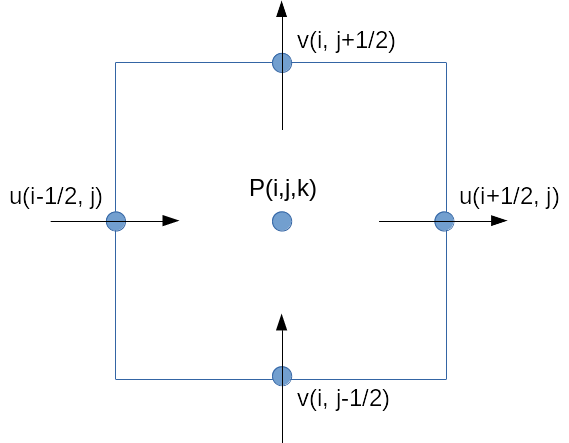
\includegraphics[width=0.5\textwidth]{mac_grid}
\caption{MAC Grid를 나태낸 그림}
\end{figure}

이젠 이것을 가지고 임의의 위치 $(x, y) \in \mathbb{R}^3$에서의 실제 속도값 $\vec{u}(x, y)$를 구할 수 있다. 예를 들어서 u에 대해서는 위치값이 1/2의 배수일 때 다음과 같이 구할 수 있다:

\begin{align*} 
  \vec{u}(i \Delta x, j \Delta x) &= (\frac{u(i-1/2, j) + u(i+1/2, j)}{2}, \frac{v(i,j+1/2) + v(i,j-1/2))}{2} \\
  \vec{u}((i+1/2) \Delta x, j \Delta x) &= (u(i,j), \frac{v(i,j-1/2) + v(i,j+1/2) + v(i+1,j-1/2) + v(i+1,j+1/2)}{4})
\end{align*}

임의의 위치에서의 Gradient 역시 쉽게 구할 수 있다:
\begin{align*}
  \vec{u}(i \Delta x, j \Delta x) &= (\frac{u(i+1/2, j) - u(i-1/2, j)}{\Delta x}, \frac{v(i,j+1/2) - v(i,j-1/2)}{\Delta x})
\end{align*}

위치값이 1/2의 배수로 떨어지지 않는 곳에서는 interpolation을 사용하여 값을 구할 수 있는데, 프로젝트에서는 bicubic interpolation을 사용한다.

\subsection{Advection: Semi-Lagrangian vs PIC method}

Semi-Lagrangian과 PIC Method (Particle-in-cell Method) 가 차이가 나는 부분은 주로 Advection Step에 있다. 

Semi-Lagrangian 방법에서는 Advection을 Eulerian 관점에서 접근해 그리드의 속도 값들에 대해 수행하게 된다. 만약에 순수히 Lagrangian 관점으로 Advection을 바라보면, i번째 particle의 현재 속력이 $\vec{v_i}$일때 위치 $\vec{x_i}$를 매 프레임마다 $\vec{x_i}(t + \Delta t) = \vec{x_i}(t) + \vec{v_i} \Delta t$로 integration을 해 주면 되므로 매우 간단하다. 하지만 Eulerian 관점에서는 속력에 대한 정보가 Grid에만 존재하므로 particle의 속력을 다른 방법을 사용해서 유추해야 한다. 그래서 Lagrangian 관점을 약간 차용해서, 시간 $t + \Delta t$에 어떠한 particle이 위치 $\vec{x}$를 지나갔다면, 그 particle은 시간 $t - \Delta t$에 위치 $\vec{x} - \vec{v} \Delta t$에 있을 것이라는 아이디어를 사용한다. 즉 $\Delta t$의 시간 뒤 위치 $\vec{x}$에서 속도는 위치 $\vec{x} - \vec{v} \Delta t$에서의 속도값으로 근사할 수 있다. (실제 프로그램의 구현에서는 $\vec{x} - \vec{v} \Delta t$와 같은 Forward-Euler가 아니라 3rd order Runge-Kutta Method를 사용한다.) \cite[p.29-33]{fluid-sim-cg}

Semi-Lagrangian 방법에서 Advection - Gravity - Pressure Solve 과정이 모두 끝난 후에는, Grid의 각 셀 값들을 유체인지, 혹은 빈 공간인지 업데이트해야 한다. 이것을 여러가지 방법으로 수행할 수 있는데, 가장 간단한 방법은 현재 유체인 셀들에 일정한 밀도로 marker particle들을 생성하고 (예를 들어 한 cell당 4개씩), 이 particle를 Pressure Solve에서 구한 velocity field를 사용해서 한 timestep동안 advection을 수행한 다음, 새로운 particle들의 위치를 가지고 level set을 만들어 유체 셀의 위치를 알아내는 방법이 있다. 혹은 다른 방법으로는 현재 유체의 영역을 나타내는 Level Set 자체에 advection을 수행하는 방법이 있다 \cite[p.57]{fluid-sim-cg}. 본 프로그램의 구현에서는 전자의 방법을 수행한다.

Semi-Lagrangian에서는 실질적으로 Advection을 그리드에서 한번, 파티클에서 한번 실행해야 한다는 단점이 있다. PIC (Particle-in-cell) Method는 이 두 가지 Advection을 하나로 통일화하는데, 시뮬레이션에서 파티클들의 위치와 속도 정보를 저장하여, advection step에서 파티클들을 직접 움직이는 방법이다. 이 방법의 문제는 Advection 후에 Gravity/Pressure Solve 를 적용하려면 넘어갈려면 파티클의 속도값을 그리드로, 반대로 Gravity/Pressure Solve 후에 Advection을 적용하려면 그리드의 속도값을 파티클로 옮기는 작업이 필요하다. PIC는 interpolation을 사용해 Eulerian 관점과 Lagrangian 관점의 속도값을 서로 변환하게 된다. 

PIC Method에서 사용하는 interpolation은 속도값들을 smoothing하는 경향이 있어, 유체에 원하지 않는 numerical dissipation을 가져오는 경향이 있다. 그래서 PIC에서 조금 수정을 가한 FLIP Method도 같이 구현했는데, FLIP에서는 그리드에서 파티클로 속도값을 가져올 때 속도값을 interpolation으로 가져오는 것이 아니라 한 프레임 동안의 속도값의 변화량을 가져오는 방식을 사용한다. FLIP의 장점으로는 PIC와 같은 dissipation이 없지만, 대신 노이즈가 증가할 수 있다는 것이다. Bridson은 PIC와 FLIP을 $\alpha$만큼의 regularization factor로 섞어서 쓰는것을 권장한다 \cite[p. 118]{fluid-sim-cg}. 즉 파티클의 속도를 구하는 식은 $\vec{u}_p^{new} = \alpha \texttt{interp}(\vec{u}_{grid}^{new}, \vec{x}_p) + (1 - \alpha) \texttt{interp}(\vec{u}_{grid}^{new} - \vec{u}_{grid}, \vec{x}_p)$로 쓸 수 있다 (왼쪽 항은 PIC, 오른쪽 항은 FLIP). 최종 프로그램에서는 서로 다른 $\alpha$값을 가지고 실험해 볼 수 있는데, $\alpha$값에 따른 유체 시뮬레이션의 변화에 대해서는 \textbf{Results} 섹션에서 다룰 것이다.

\subsection{Pressure Solve}

\textbf{MAC Grid} 섹션에서의 공식들을 사용해 (2)의 incompressibility 조건과 (5)의 Pressure solve 공식을 불연속적인 버젼으로 옮길 수 있다. 식을 정리하면 다음과 같이 나온다:

\begin{equation}
  \frac{\Delta t}{\rho} (\frac{4p_{i,j} - p_{i+1,j} - p_{i-1,j} - p_{i,j+1} - p_{i,j-1}}{\Delta x^2}) = -\frac{u_{i+1/2,j} - u_{i-1/2,j} + u_{i,j+1/2} - u_{i,j-1/2}}{\Delta x}
\end{equation}

이젠 이 식을 $Ap = b$꼴의 linear system으로 변환할 수 있다. 다만 조심해야 할 것은 현재 유체의 상황을 반영하여 경계조건을 주어야 하는데, 첫 번째는 비어있는 셀들에는 압력값이 0 ($p = 0$)이라는 Dirichlet 경계조건이다. 두 번째는 유체가 고체 벽을 통과하지 못한다는 것($\Delta t / \rho \cdot \partial_x p = u - u^{solid}$)을 나타내는 Neumann 경계조건이다. \cite[p. 69-70]{fluid-sim-cg} 이 제한조건들을 적용함으로 인해 행렬 $A$가 바뀌게 된다.

이젠 linear system $Ap = b$를 풀기 위해서는 MICCG (Modified Incomplete Cholesky Conjugate Gradient) 방법을 사용한다. 이것은 선형 시스템을 푸는 대표적인 방법 중 하나인 Conjugate Gradient에 근사를 가해 좀 더 빠르게 만든 것으로, Bridson의 책 \cite[p.79]{fluid-sim-cg}에 잘 설명되어 있다.

\subsection{Level Set Method}

Pressure Solve 과정을 수행하는 데 중요한 부분 중에 하나가 어떤 위치에 유체 안쪽 혹은 바깥쪽에 있는지를 판별하는 것이다. 가장 간단하게 이것을 해결하는 방법은 파티클이 걸쳐있는 셀들을 모두 유체로 마킹하고 그렇지 않은 것은 빈 공간으로 마킹하는 것이다. 하지만 이 방법을 사용했을 때에는 파티클들의 수가 많지 않을 때 생기는 유체 내의 작은 기포 (빈 공간)를 매꾸지 못하여 유체의 내부에서 원하지 않는 유속이 생긴다는 문제를 발견하였다.

그래서 최종 프로그램에서는 Level Set Method를 통해 signed distance function을 구하는 방법을 사용할 것이다. Signed distance function은 특정 지점에서 가장 가까운 유체 파티클까지의 거리를 나태낸다. (이름에 signed가 붙은 이유는 유체 내부에서는 음수가 되기 때문이다). 이 함수를 $\phi: \mathbb{R}^3 \rightarrow \mathbb{R}$이라고 하면, Eikonal equation ($|\nabla \phi| = 1$)를 만족하게 된다. 프로그램에서는 Closest Point Method \cite[p. 11]{dist-function}로 유체 바깥과 경계의 $\phi$값들을 구한 다음, Fast Sweeping Method\cite{fast-sweeping}을 사용하여 유체 안쪽의 $\phi$값들도 구하게 된다. (자세한 방법은 \cite[p.49-p.56, p.126]{fluid-sim-cg} 참조.) Eikonal equation의 해 $\phi$를 찾아내고 나면, 특정 지점에서 $\phi$값이 음수인지 양수인지를 판별하여 유체의 안과 바깥을 구분한다.

프로그램에서 Level Set Method는 유체의 안과 바깥을 구분하는 것 이외에 다른 용도로도 쓰인다. Pressure solve를 진행할 때 빈 공간의 압력이 0이라는 Neumann 경계조건을 적용했는데, 이것은 유체의 경계에서 문제가 될 수 있다. Level-Set의 경계가 셀 사이를 지나가면서, 그리드에서 부분적으로만 채워져 있는 유체 셀들이 존재할 수 있기 때문에, 이 경우에는 이 셀들에 존재할 수 있는 압력에 대해 보정을 해 주어야 한다. 이것을 유체의 Level Set 함수를 사용해서 보정하는 방식이 Ghost Fluid Method인데, 이것을 사용하면 그리드로 인해 유체 시뮬레이션에서 생기는 artifact를 줄일 수 있다. \cite[p.127-129]{fluid-sim-cg}

\subsection{Summary}

즉 시뮬레이션의 메인 루프를 다음과 같이 pseudocode로 쓸 수 있다:

\begin{verbatim}
loop:
  if (Semi-Lagrangian method):
    Create level set for fluid (and find fluid cells using the level set)
    Advect grid velocities using Semi-Lagrangian advection 
    Apply gravity to velocity field
    Solve for pressure and update velocity field
    Advect marker particles
  else if (PIC method):
    Create level set for fluid (and find fluid cells using the level set)
    Move velocities from particles to grid
    Apply gravity to velocity field
    Solve for pressure and update velocity field
    Move velocities from grid to particles
    Advect particles according to particle velocities
\end{verbatim}

\subsection{Implementation Details}

본 시뮬레이션은 C++로 구현하였으며, 여러 개의 코어에서 병렬화를 하기 위해 OpenMP를 사용하였다. (즉 OpenMP를 지원하는 컴파일러가 필요하다.) 프로그램 개발 환경은 Linux, 컴파일러는 Clang을 사용하였다. (코드는 https://github.com/lasagnaphil/fluid-sim에서 확인할 수 있다.) 개발에 사용된 라이브러리는 다음과 같다.

\begin{itemize}
  \item OpenGL (그래픽)
  \item SDL (창 생성/입출력 관련)
  \item IMGUI (UI 관련된 부분)
  \item MathFu (수학 라이브러리)
\end{itemize}

시뮬레이션의 성능을 높이기 위해서 여러가지 방법을 사용했는데, 일부 연산을 가속화시키기 위해 AVX/FMA SIMD intrinsics를 사용했다. (이것의 사용 유무를 CMake 빌드 세팅에서 \texttt{USE\_SIMD} 옵션으로 제어할 수 있다.) 예를 들어서, 연산에 많이 사용되는 함수 중 하나인 bicubic linear interpolation 함수, 그리고 pressure solve에서 자주 사용되는 벡터 간의 multiply-add 연산이 최적화 대상 중에 있었다.  그리고 OpenMP를 사용하여 유체 시뮬레이션 코드 중 병렬화가 편이한 부분 (loop index 사이에 dependency가 없는 for loop)을 여러 쓰레드에서 돌릴 수 있도록 했다.

사용자는 UI를 통해 중력의 크기 (x축과 y축)과 $\alpha$값 (PIC/FLIP의 regularization factor)를 바꿀 수 있고, 시뮬레이션에 관련된 중요한 값들 (현재 시간, 평균 압력, 평균 속도) 등을 볼 수 있다. 그리고 좌클릭 드래그를 통해 유체의 한 지점의 속도를 바꿀 수 있고, 우클릭 드래그를 통해 시뮬레이션 전체의 중력을 바꿀 수 있다.

또한 사용자는 현재 유체에 해당되는 셀의 위치 뿐만 아니라, 사용하고 있는 파티클의 위치와 속도 벡터를 볼 수 있다. 해당하는 옵션을 클릭하면 각 셀의 압력의 크기, 그리고 level set의 모습도 볼 수 있다.

\section{Results}

3가지의 초기 상태 (물 particle의 초기 위치) 에 대해서 시뮬레이션을 수행해 보았다.$\Delta t$ = 0.033s, $\Delta x = 0.02m$, 그리드 크기=128x128, 셀 당 입자 개수 4개, 중력 9.81$m/s^2$으로 고정하고 다음 실험들을 진행하였다. 초기 상태는 다음과 같이 세 종류를 주었다:

\begin{enumerate}[label=\Alph*.]
  \item 모자 모양으로 되어 있는 배열 형태.
  \item 물 전체가 한쪽으로 기울어져 있는 형태.
  \item 정육면체의 모양의 물 영역이 떨어지는 형태.
\end{enumerate}

각각의 초기 상태에 대한 스크린샷은 다음과 같다.

\begin{figure}[h]
  \centering
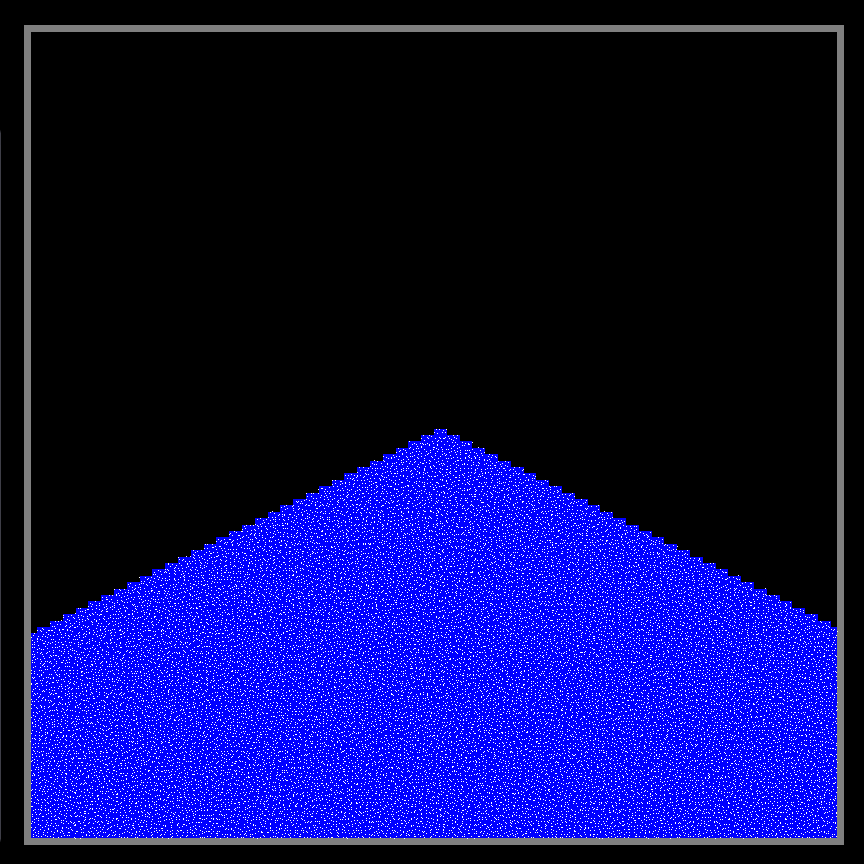
\includegraphics[width=0.25\textwidth]{init_state_1}
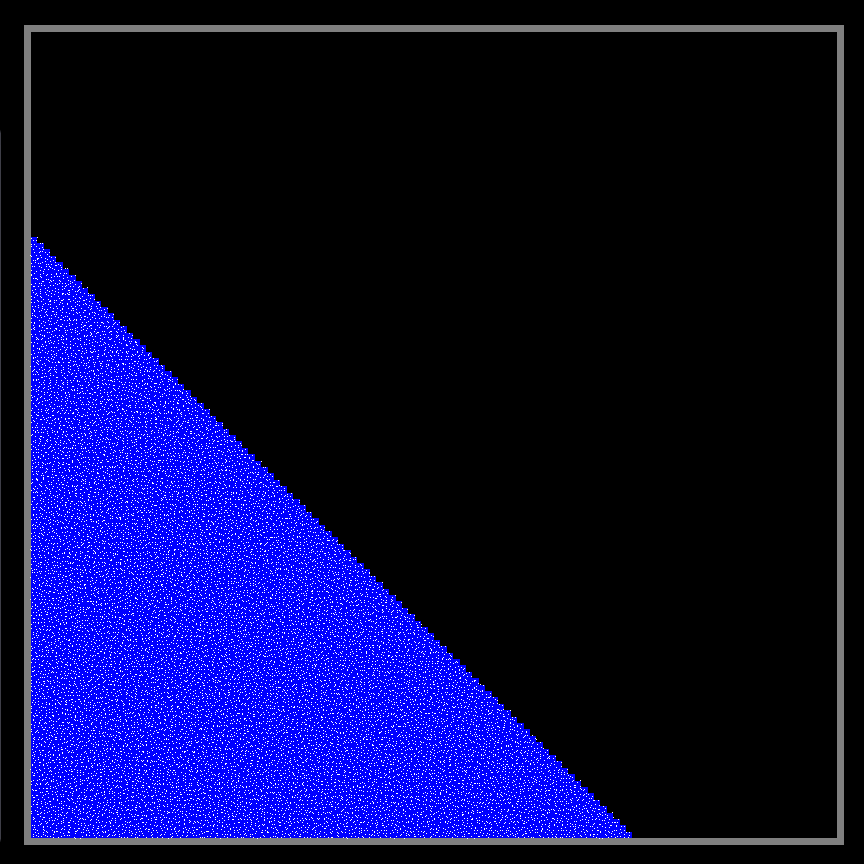
\includegraphics[width=0.25\textwidth]{init_state_2}
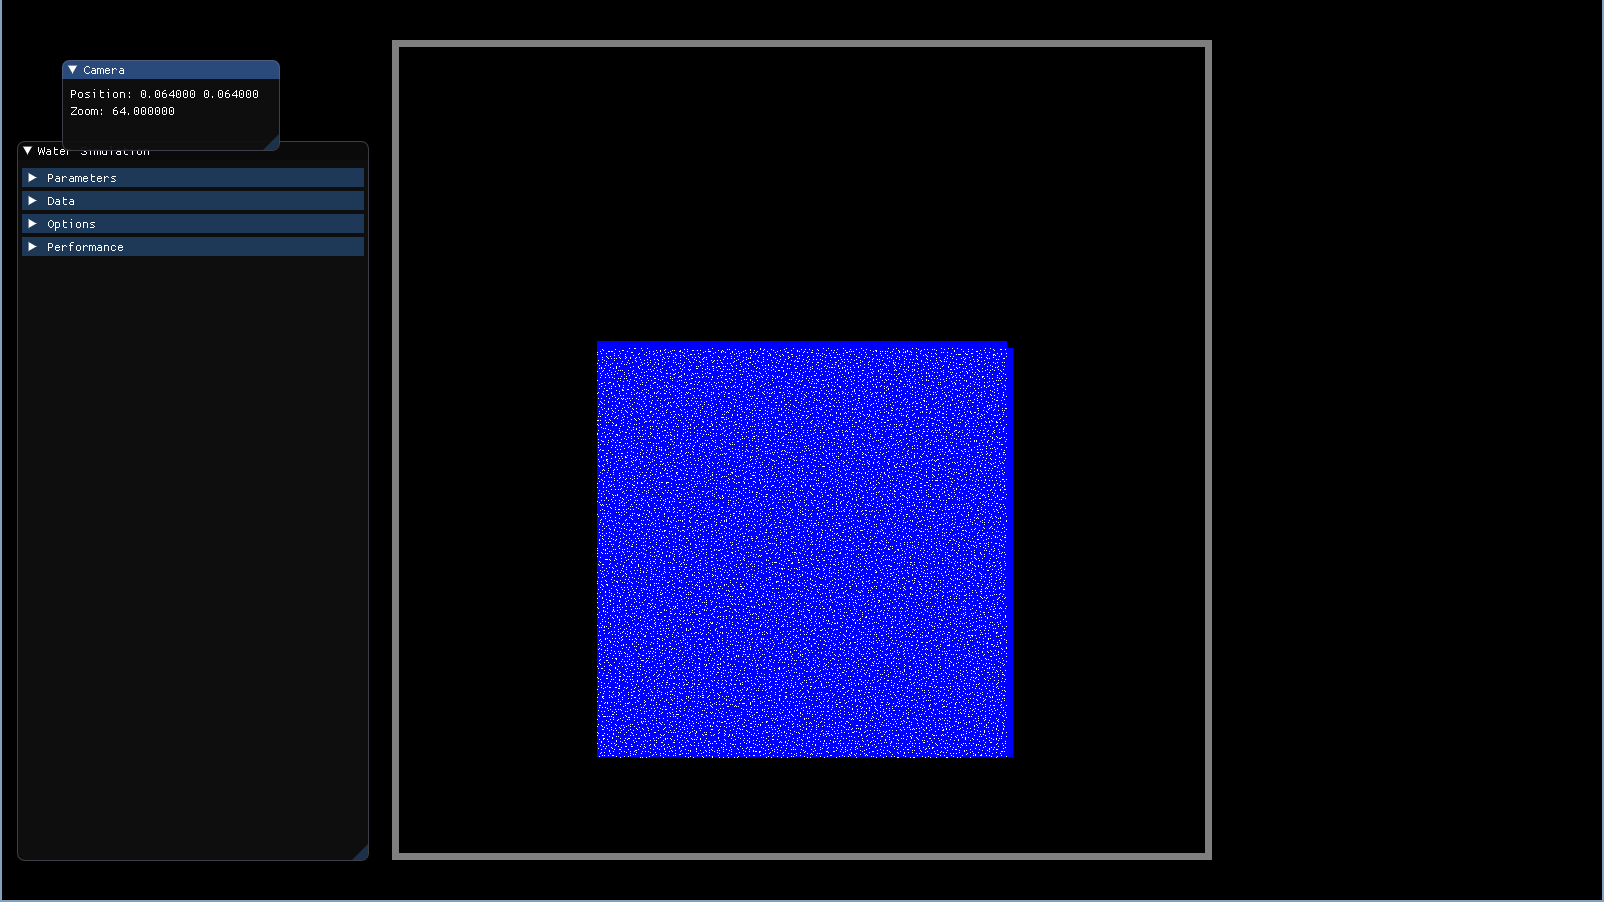
\includegraphics[width=0.25\textwidth]{init_state_3}
  \caption{3가지의 초기 상태를 나타낸 사진.}
  \label{fluid-init-state}
\end{figure}

\subsection{Realism}

일단 초기상태 A, B, C 상태에서 유체를 가만히 두었을 때 Semi-Lagrangian (위)와 PIC (아래) 유체의 변화를 보았다. (\Delta t = 0.033s, \Delta x = 0.02m)

\begin{figure}[h!]
  \centering
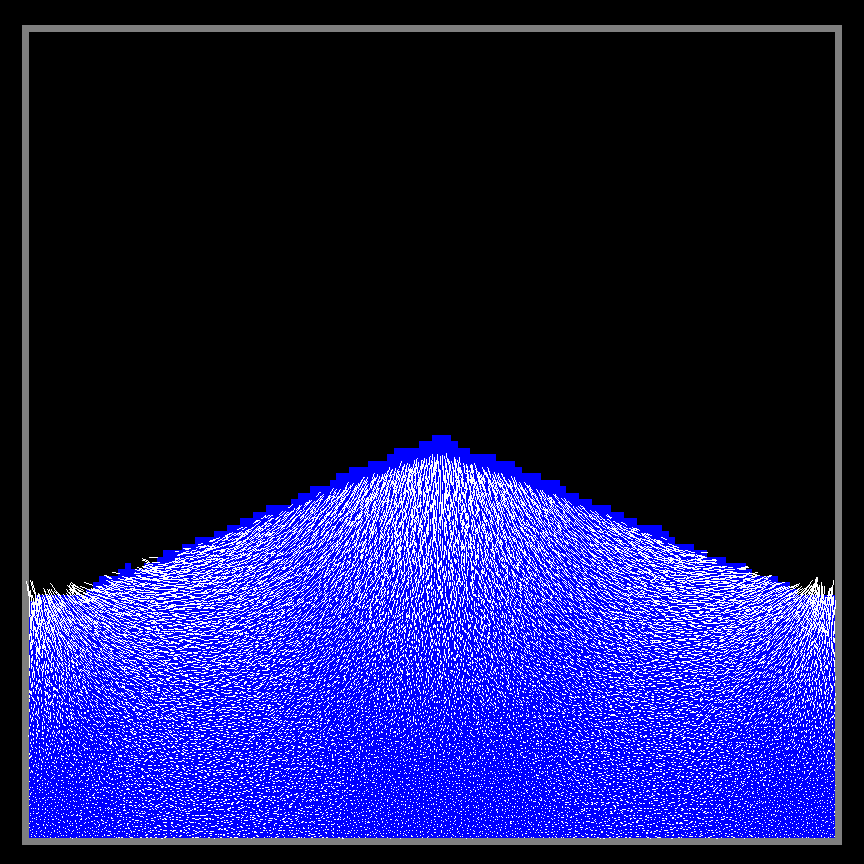
\includegraphics[width=0.20\textwidth]{semilag-state-a/img1}
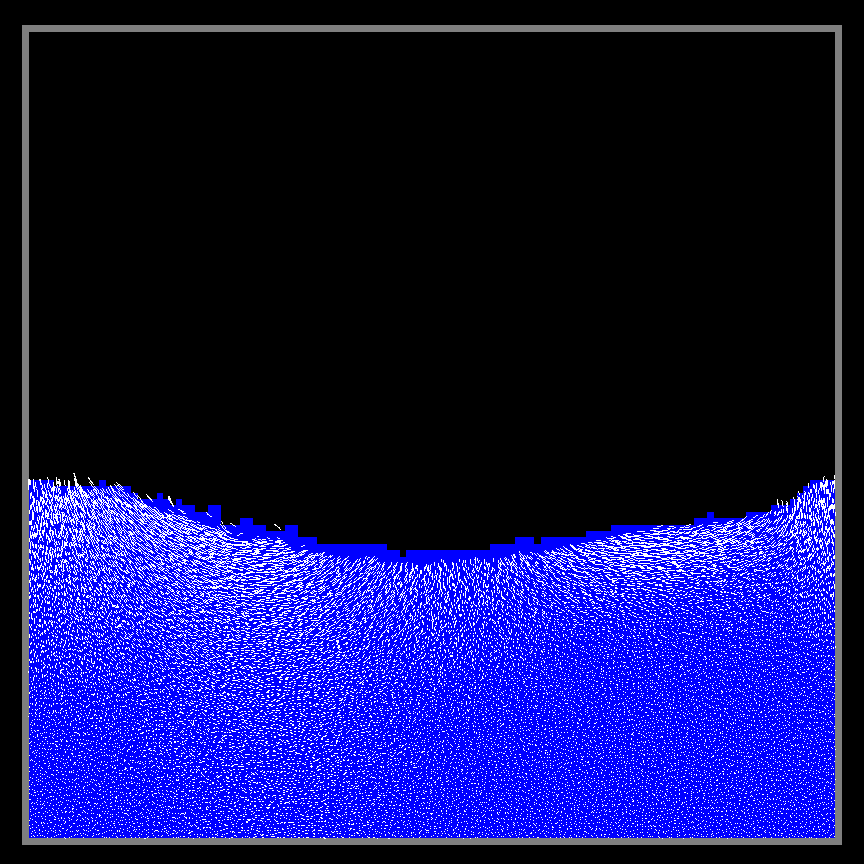
\includegraphics[width=0.20\textwidth]{semilag-state-a/img2}
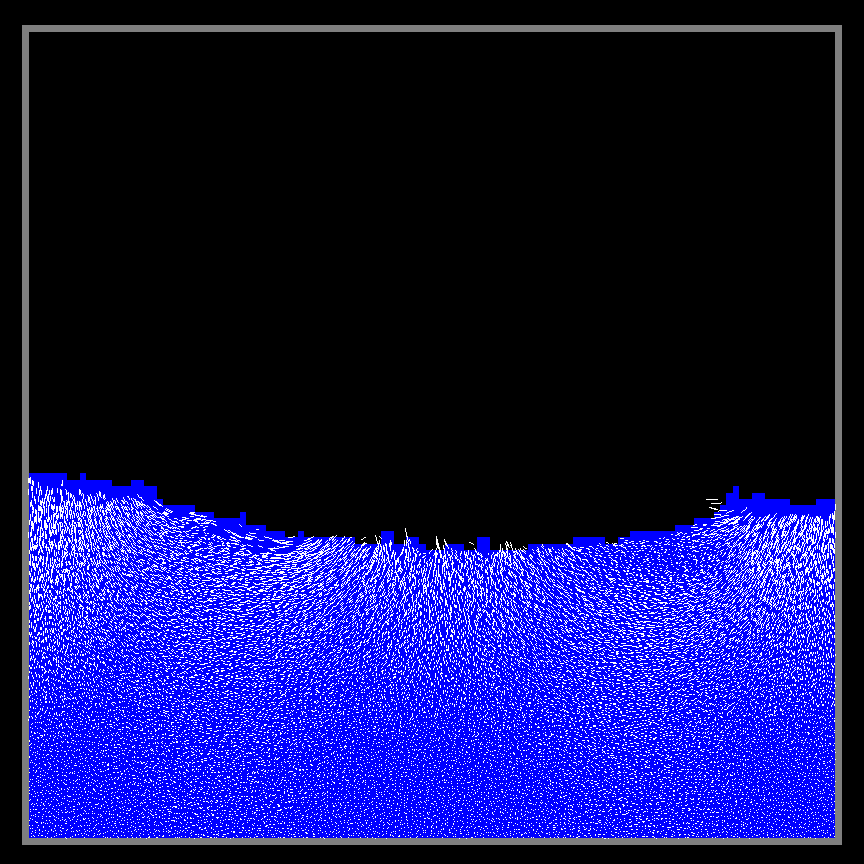
\includegraphics[width=0.20\textwidth]{semilag-state-a/img3}
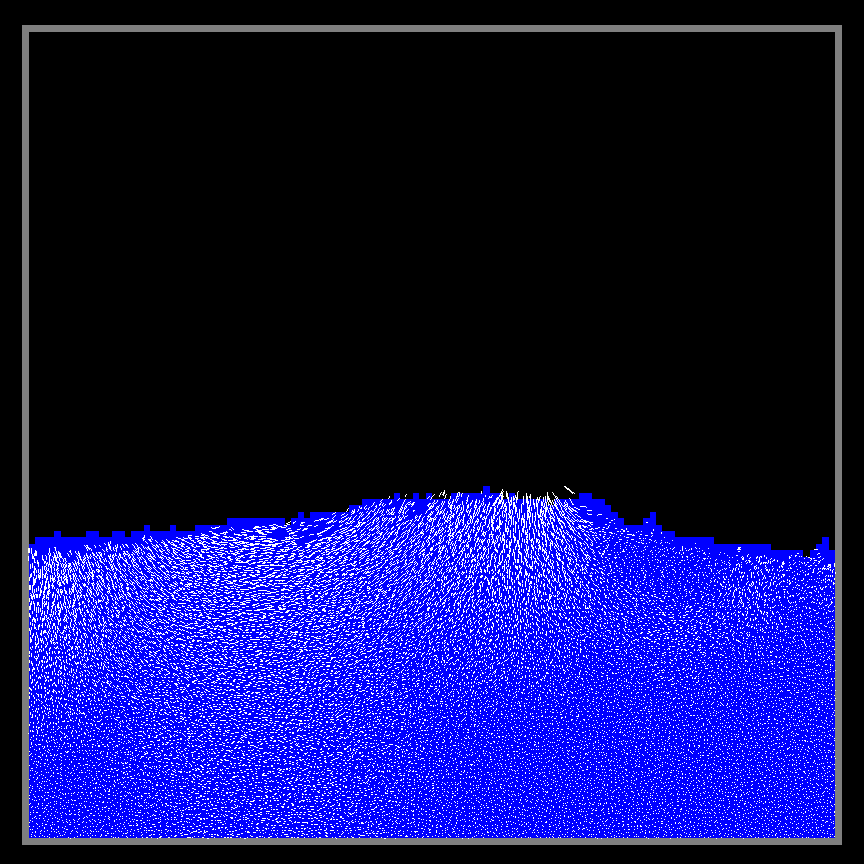
\includegraphics[width=0.20\textwidth]{semilag-state-a/img4}

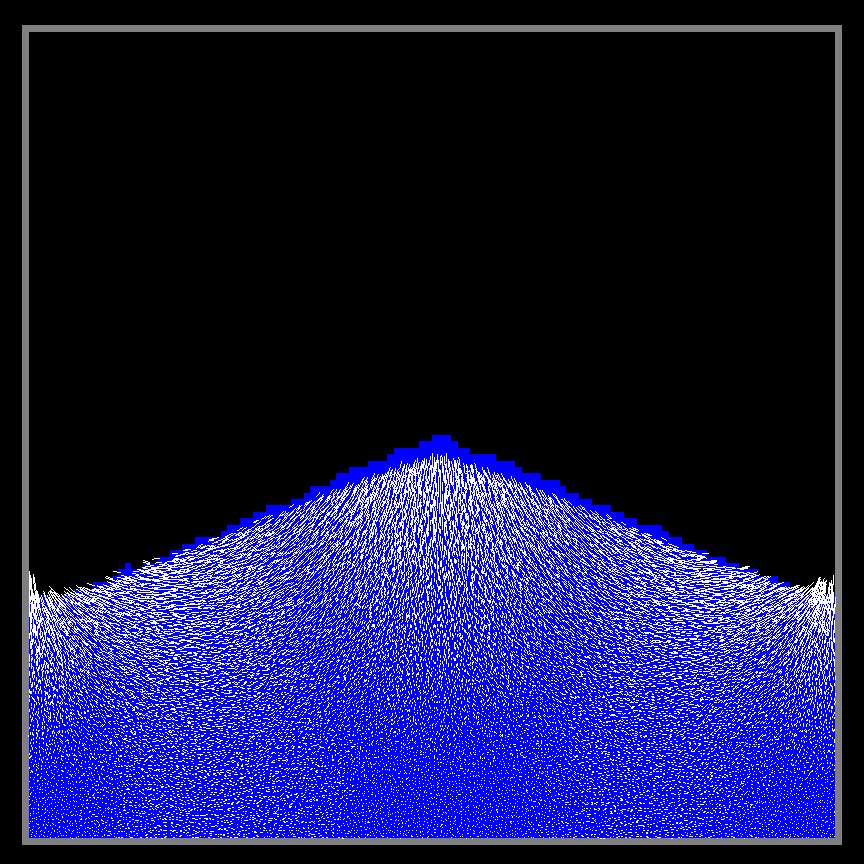
\includegraphics[width=0.20\textwidth]{pic-state-a/img1}
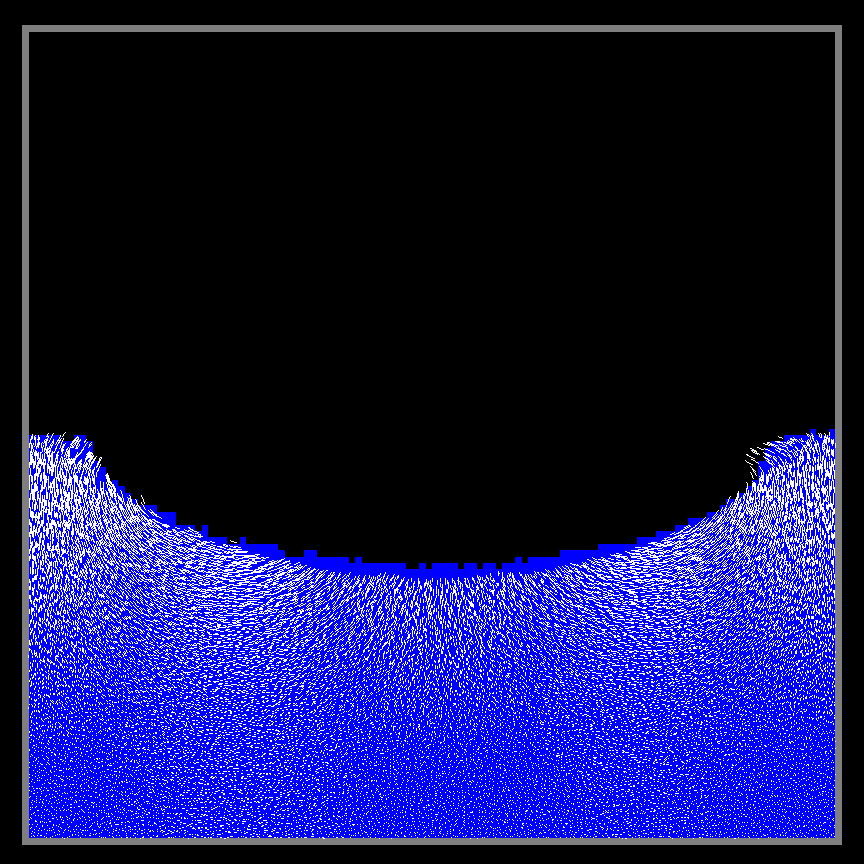
\includegraphics[width=0.20\textwidth]{pic-state-a/img2}
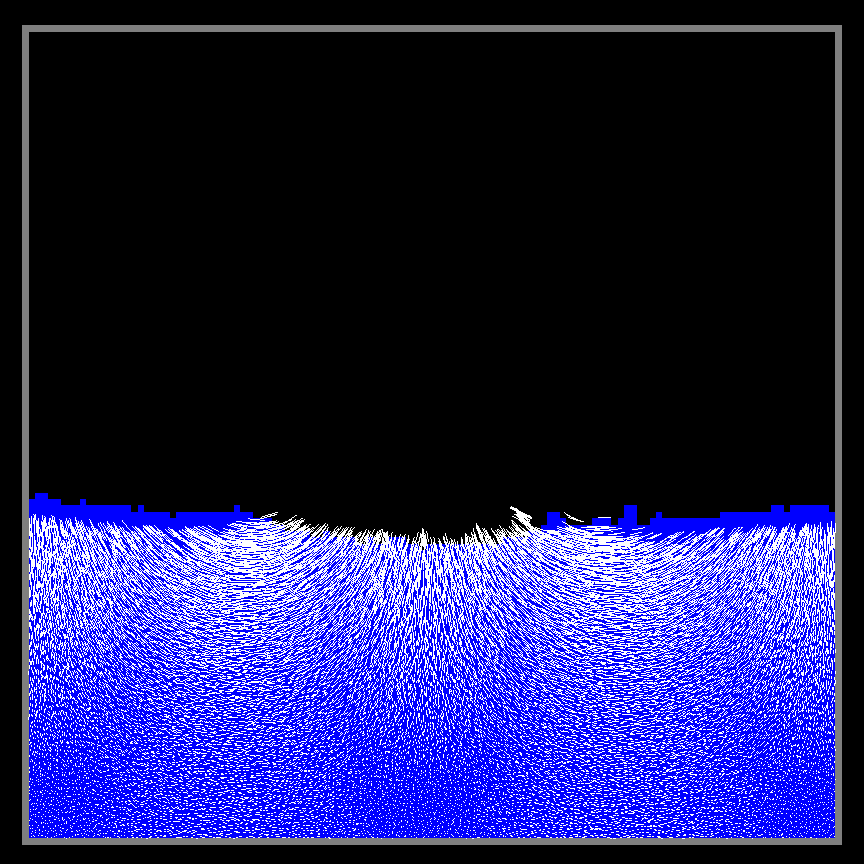
\includegraphics[width=0.20\textwidth]{pic-state-a/img3}
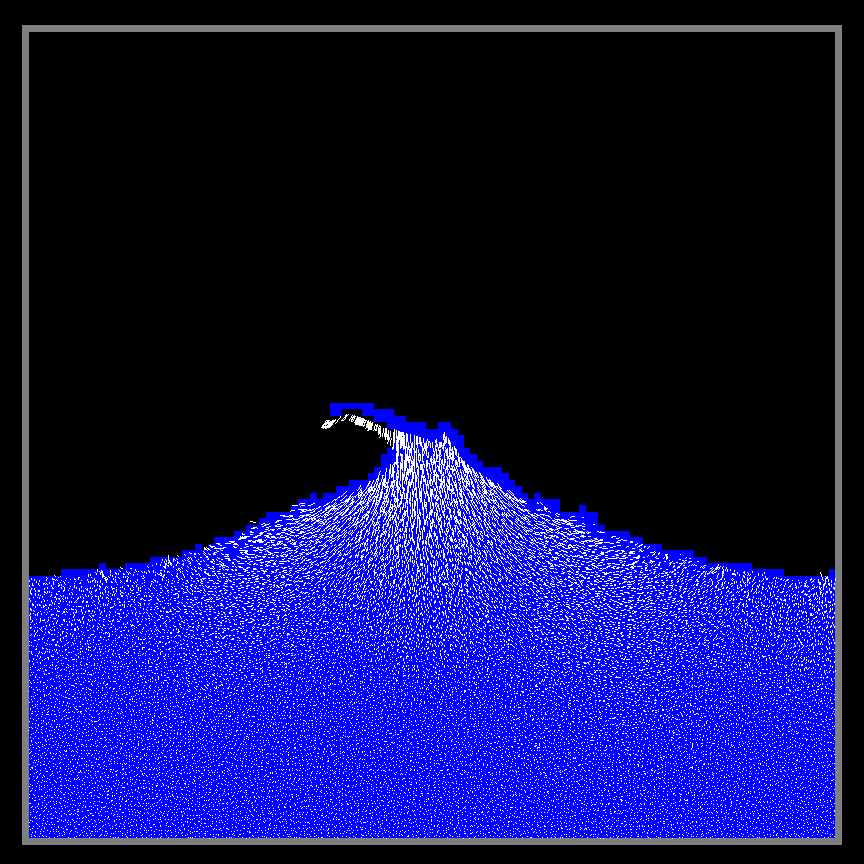
\includegraphics[width=0.20\textwidth]{pic-state-a/img4}
  \caption{초기상태 A에서 시작했을 때. 위는 Semi-Lagrangian, 아래는 PIC ($\alpha$ = 1.0)}
  \label{fluid-a}
\end{figure}

\begin{figure}[h!]
  \centering
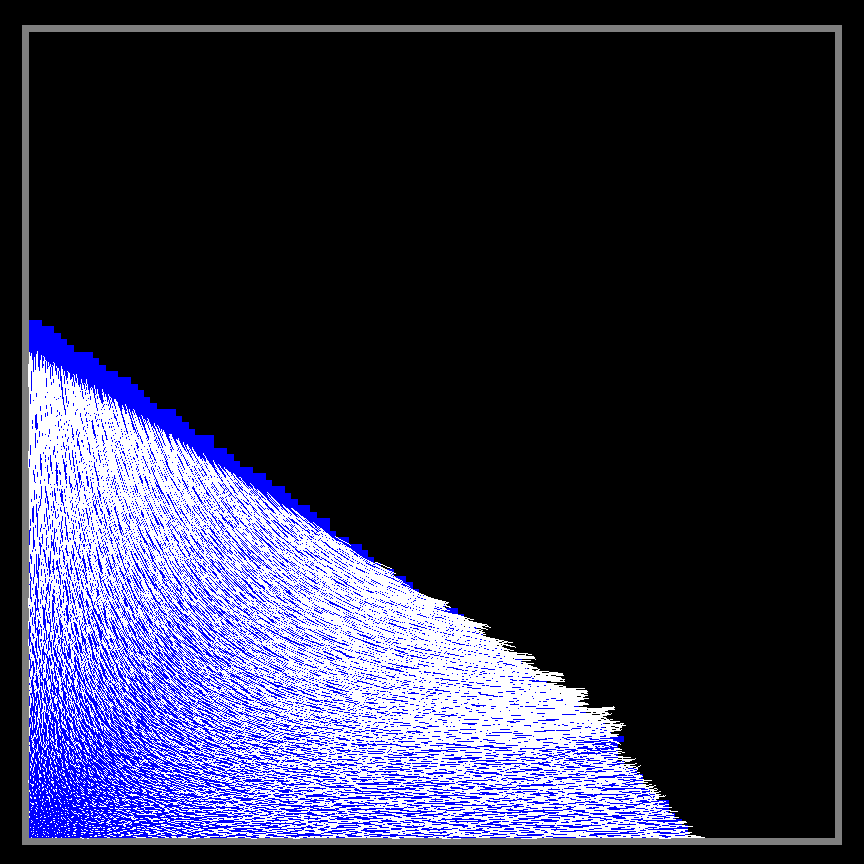
\includegraphics[width=0.20\textwidth]{semilag-state-b/img1}
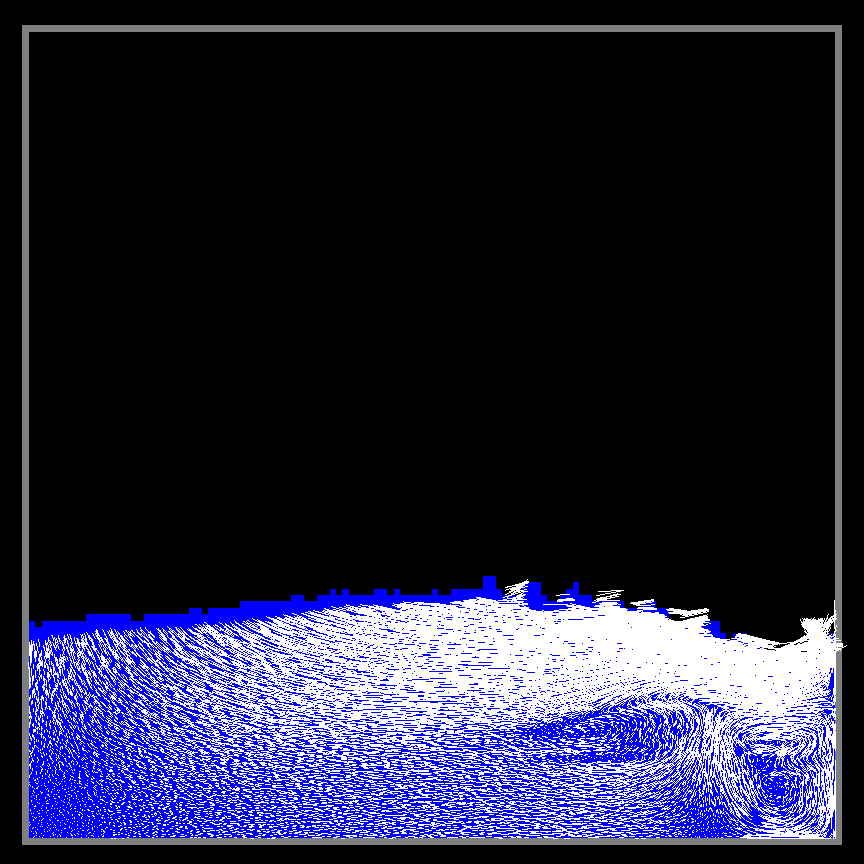
\includegraphics[width=0.20\textwidth]{semilag-state-b/img2}
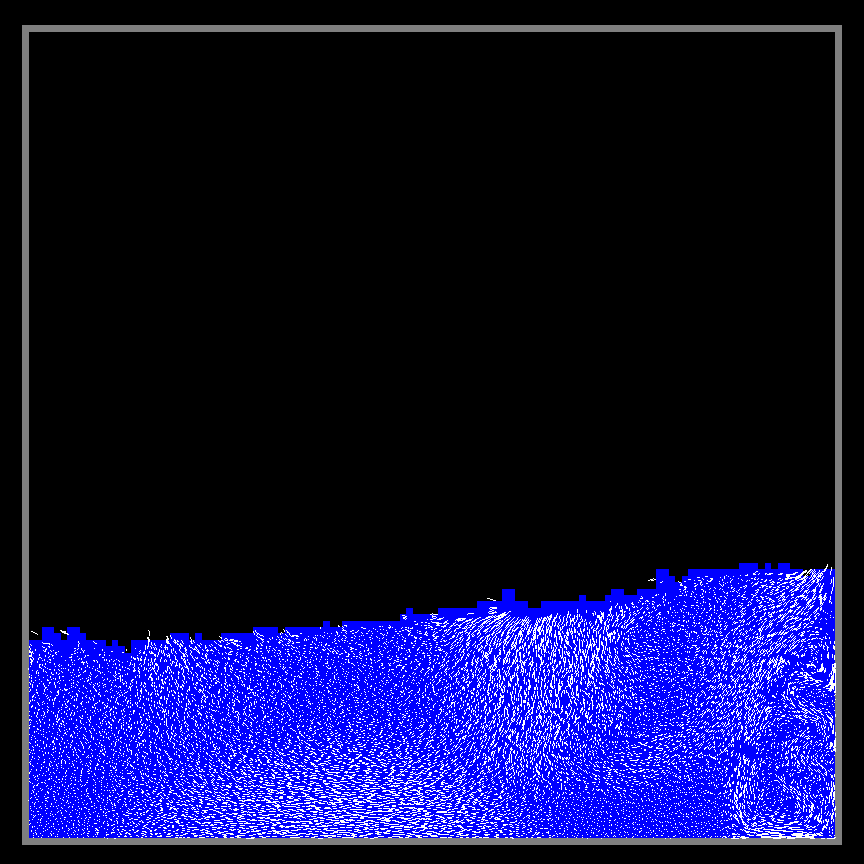
\includegraphics[width=0.20\textwidth]{semilag-state-b/img3}
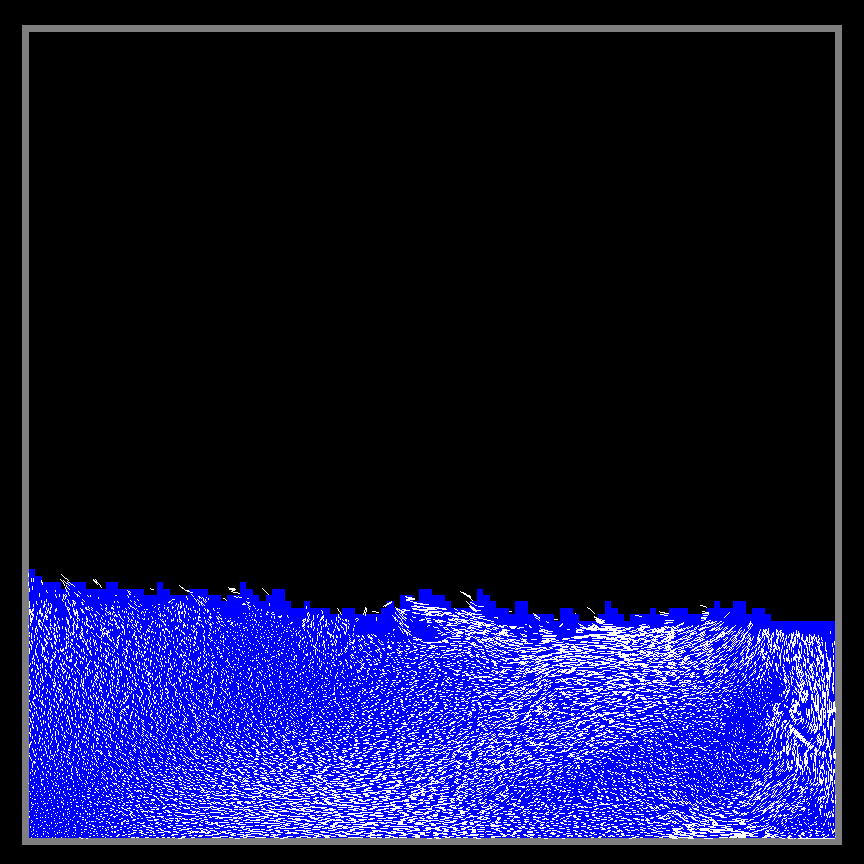
\includegraphics[width=0.20\textwidth]{semilag-state-b/img4}

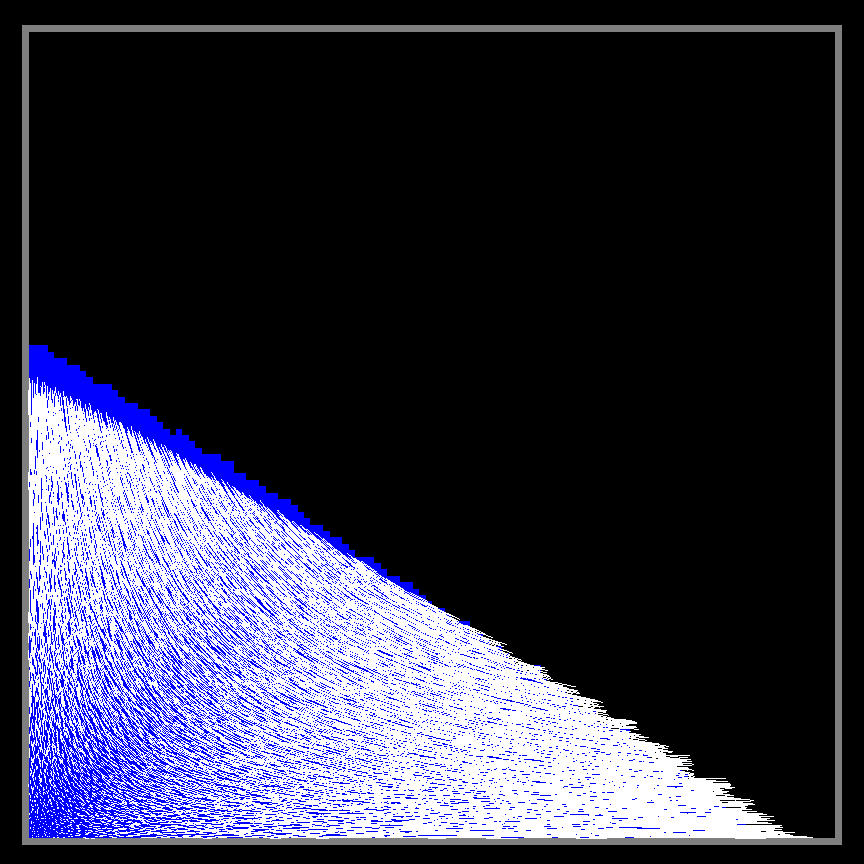
\includegraphics[width=0.20\textwidth]{pic-state-b/img1}
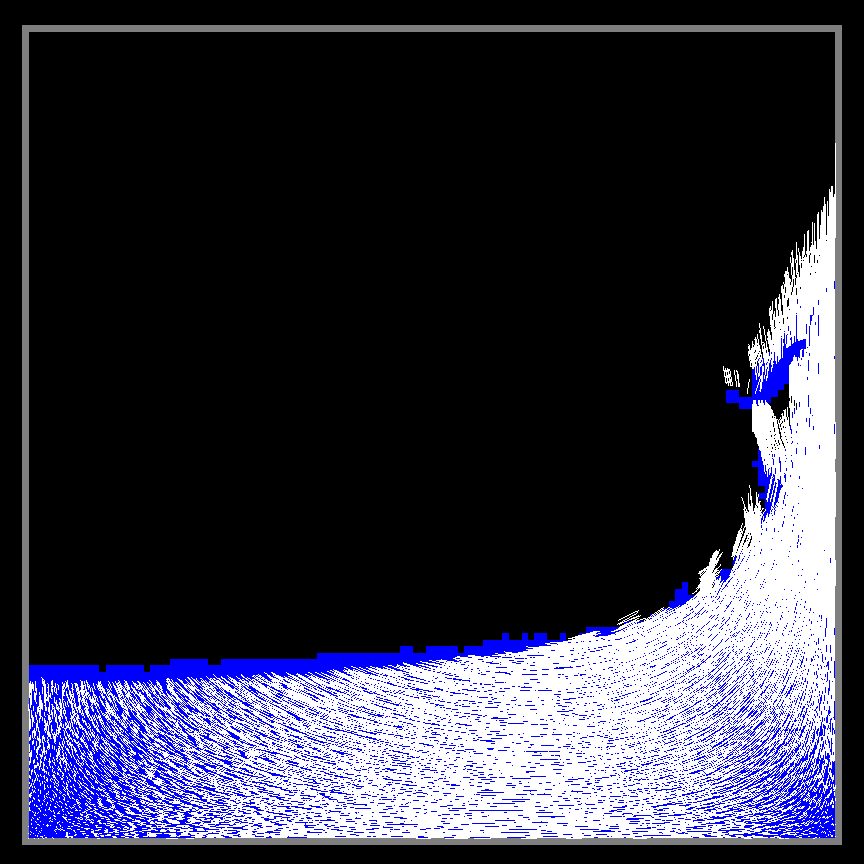
\includegraphics[width=0.20\textwidth]{pic-state-b/img2}
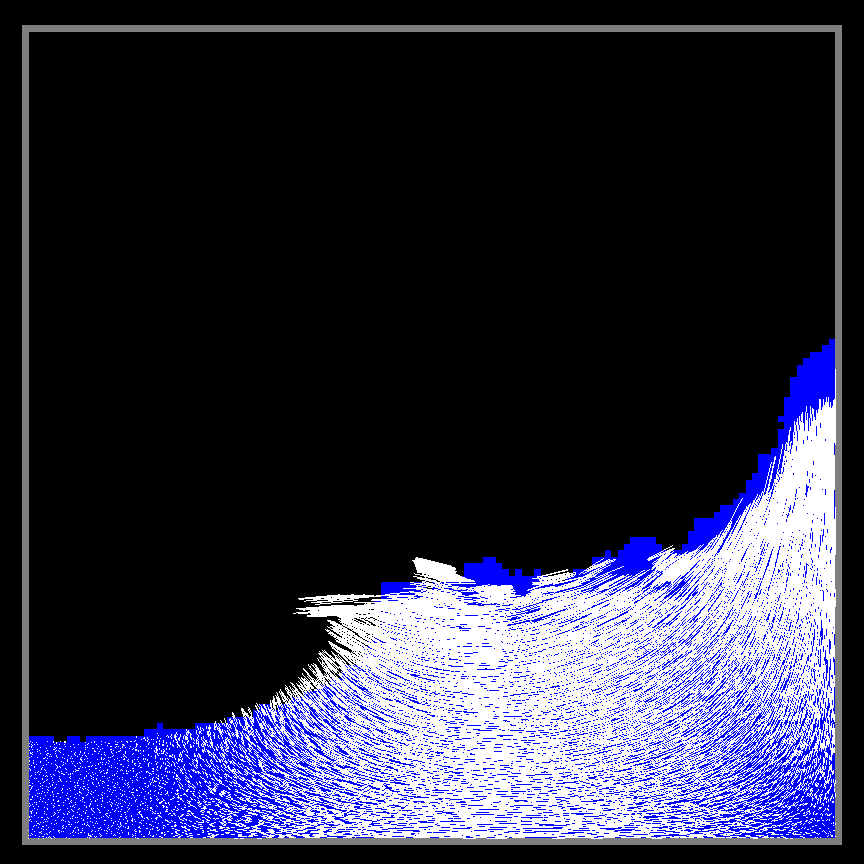
\includegraphics[width=0.20\textwidth]{pic-state-b/img3}
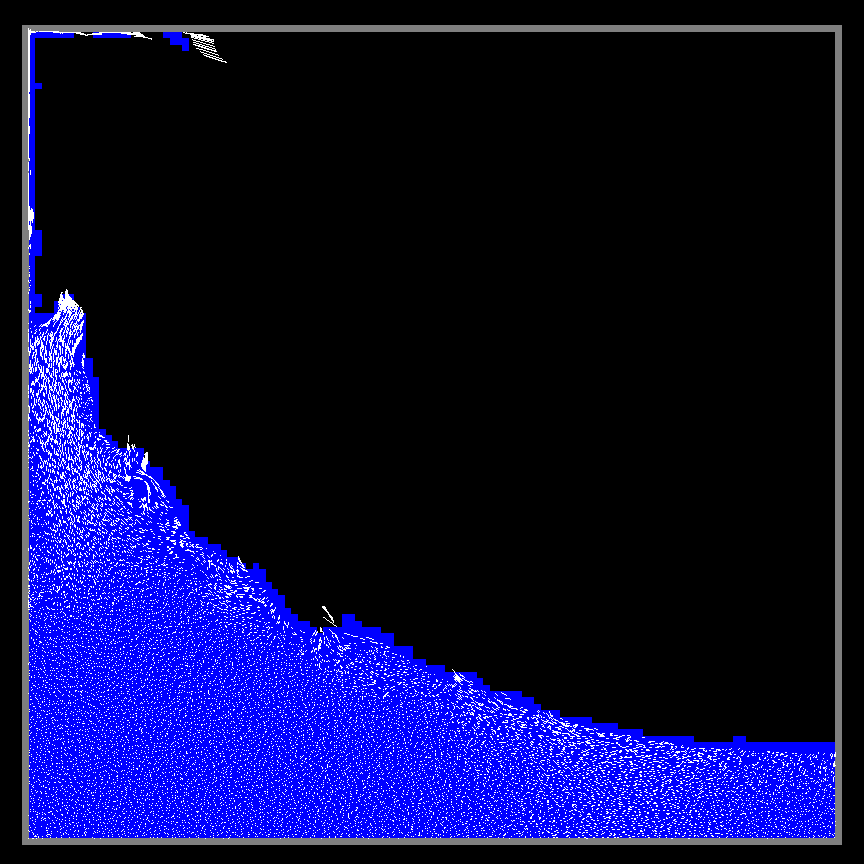
\includegraphics[width=0.20\textwidth]{pic-state-b/img4}
  \caption{초기상태 B에서 시작했을 때. 위는 Semi-Lagrangian, 아래는 PIC ($\alpha$ = 1.0)}
  \label{fluid-b}
\end{figure}

\clearpage

\begin{figure}[h!]
  \centering
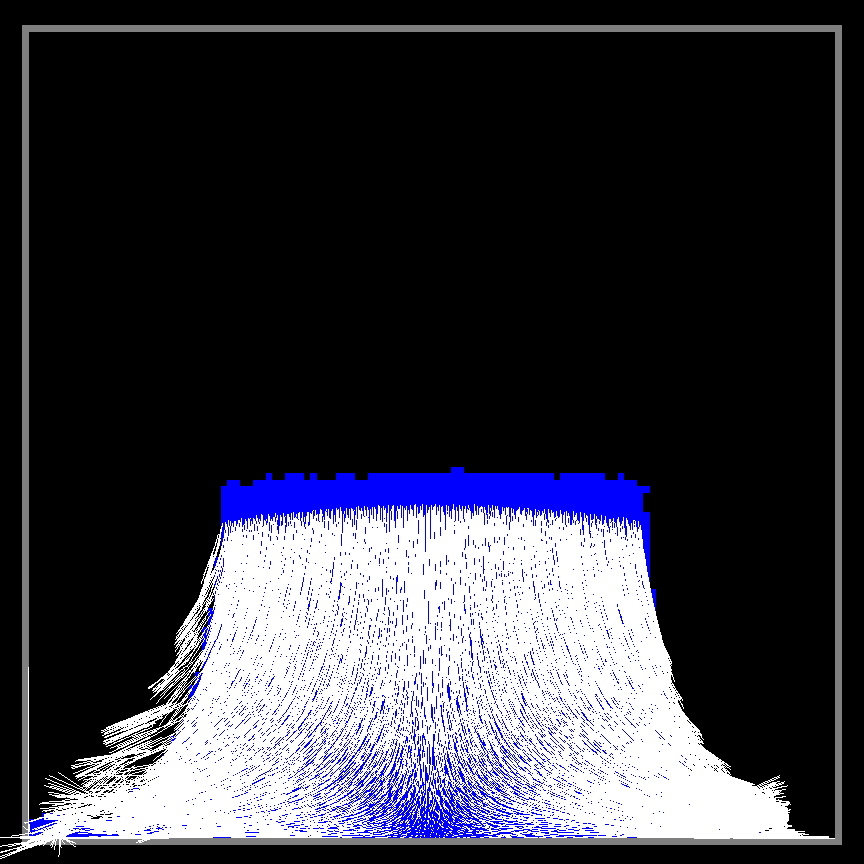
\includegraphics[width=0.20\textwidth]{semilag-state-c/img11}
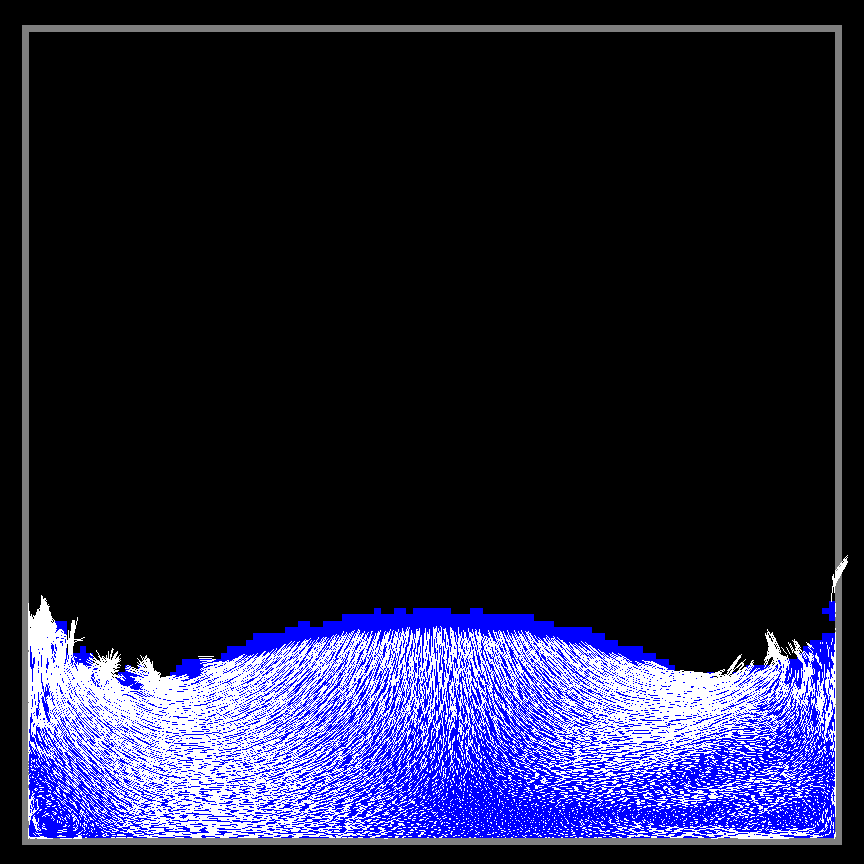
\includegraphics[width=0.20\textwidth]{semilag-state-c/img2}
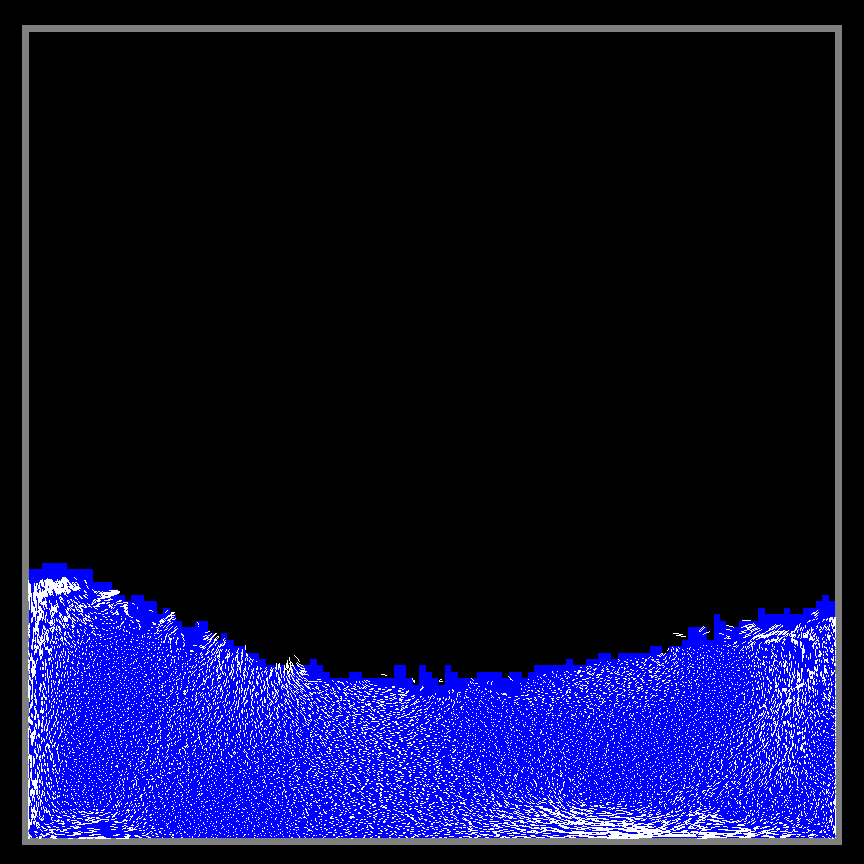
\includegraphics[width=0.20\textwidth]{semilag-state-c/img3}
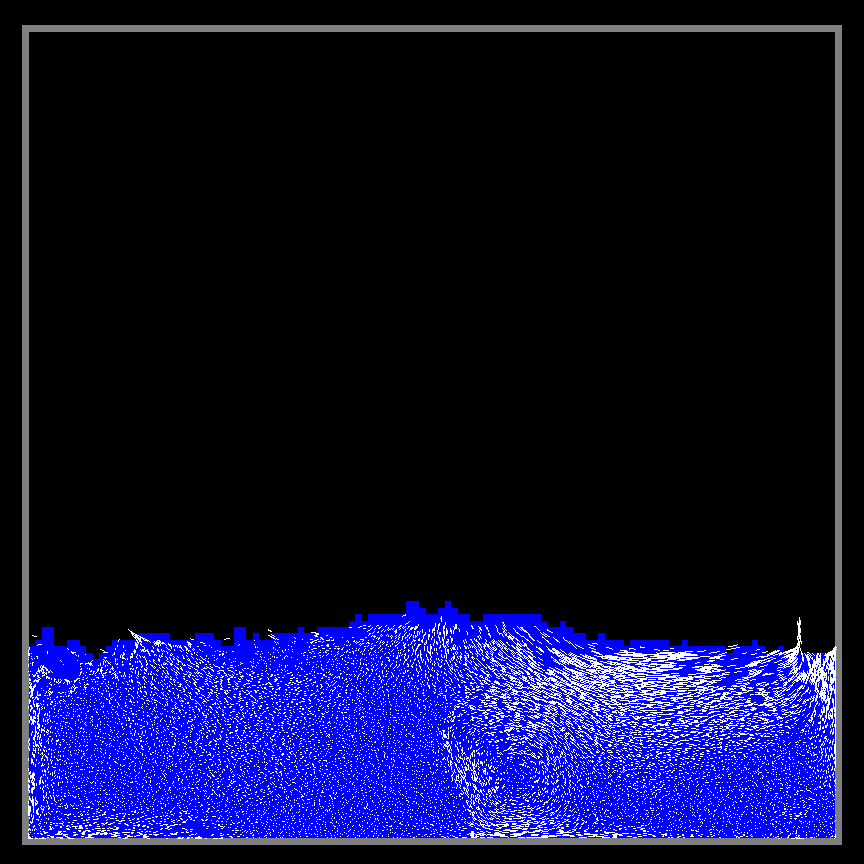
\includegraphics[width=0.20\textwidth]{semilag-state-c/img4}

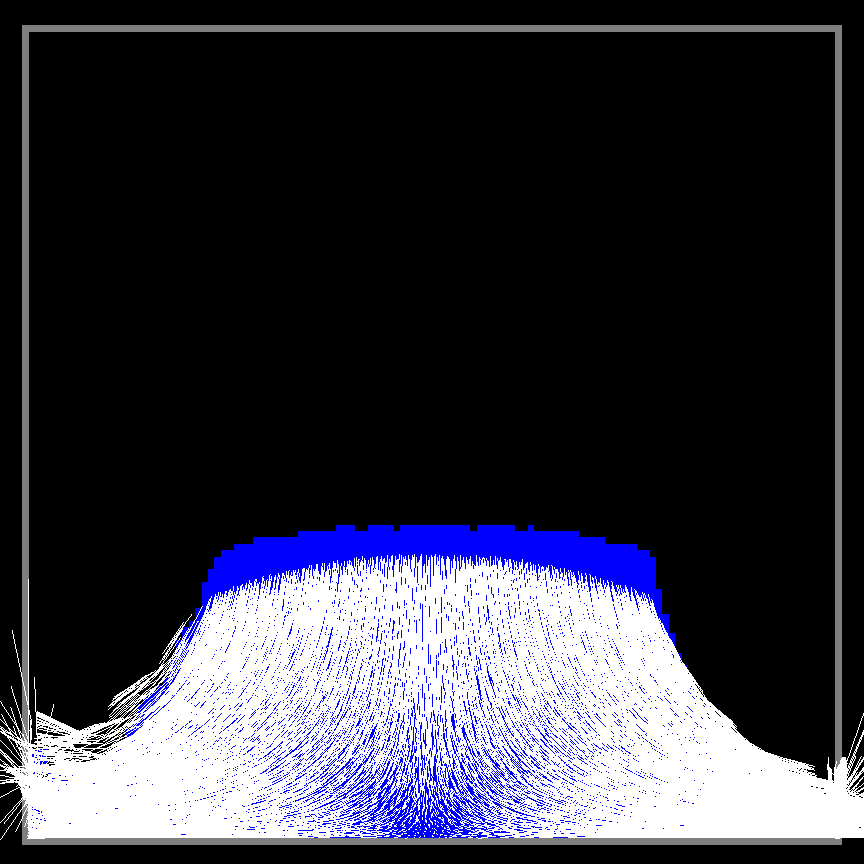
\includegraphics[width=0.20\textwidth]{pic-state-c/img1}
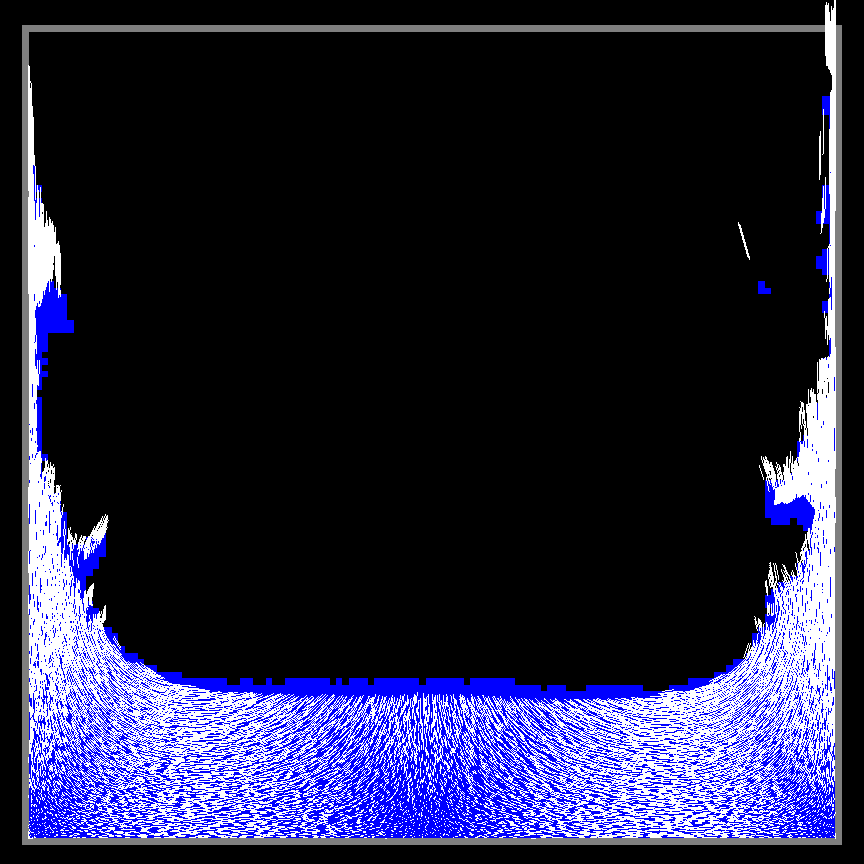
\includegraphics[width=0.20\textwidth]{pic-state-c/img2}
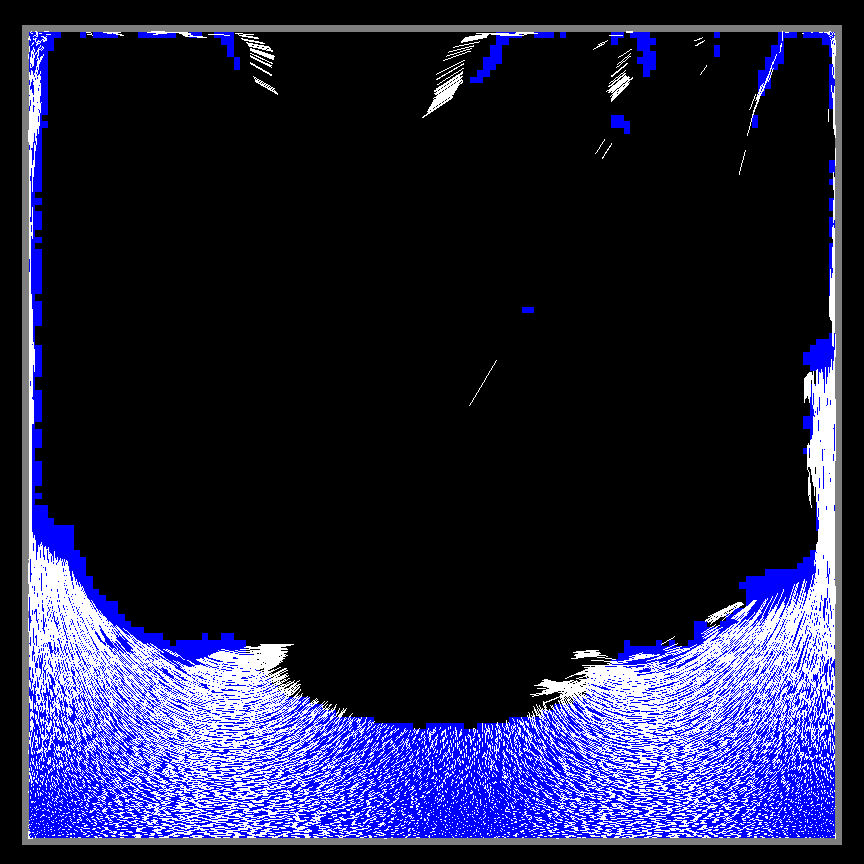
\includegraphics[width=0.20\textwidth]{pic-state-c/img3}
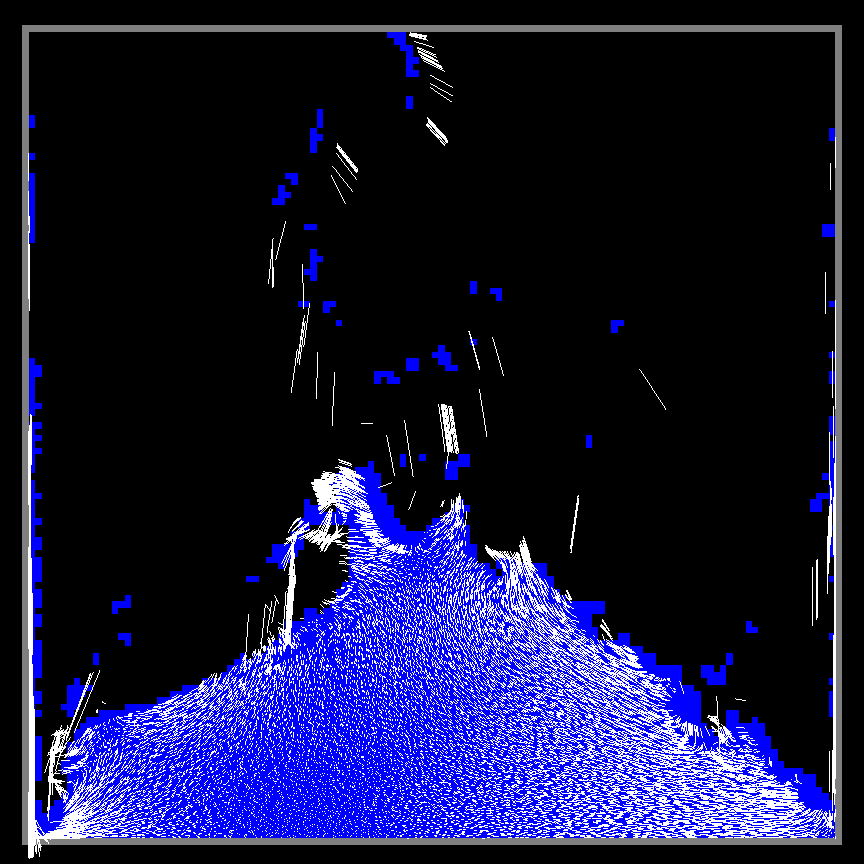
\includegraphics[width=0.20\textwidth]{pic-state-c/img4}
  \caption{초기상태 C에서 시작했을 때. 위는 Semi-Lagrangian, 아래는 PIC ($\alpha$ = 1.0)}
  \label{fluid-c}
\end{figure}

Figure \ref{fluid-a}, \ref{fluid-b}, \ref{fluid-c} 를 보았을 때, 결과적으로 PIC 방법이 Semi-Lagrangian 방법에 비해 좀 더 생동감 있는 모습을 보였다. 즉 Semi-Lagrangian은 잔잔한 물을 시뮬레이션하고 싶을 때, PIC는 더욱 유동적인 물을 시뮬레이션하고 싶을 때 사용하면 좋을 것이다.

\begin{figure}[h]
  \centering
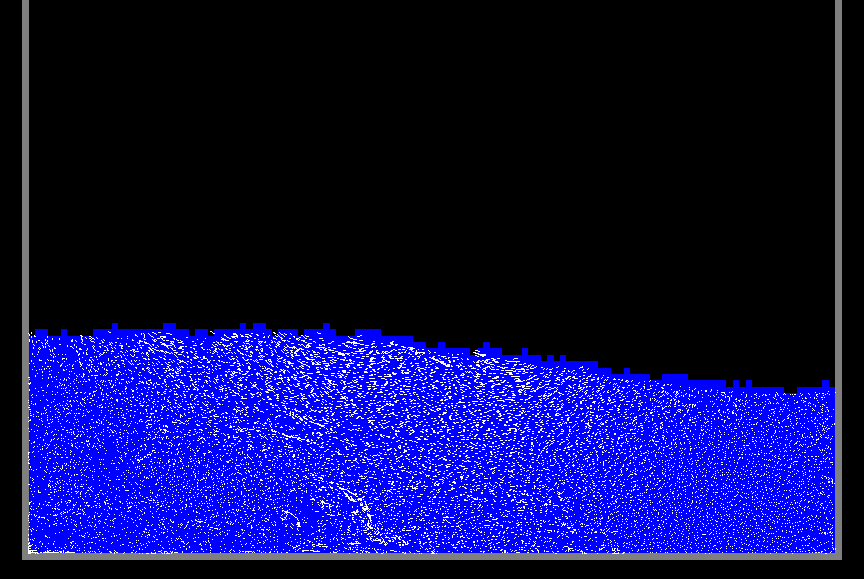
\includegraphics[width=0.40\textwidth]{pic-perturb-1}
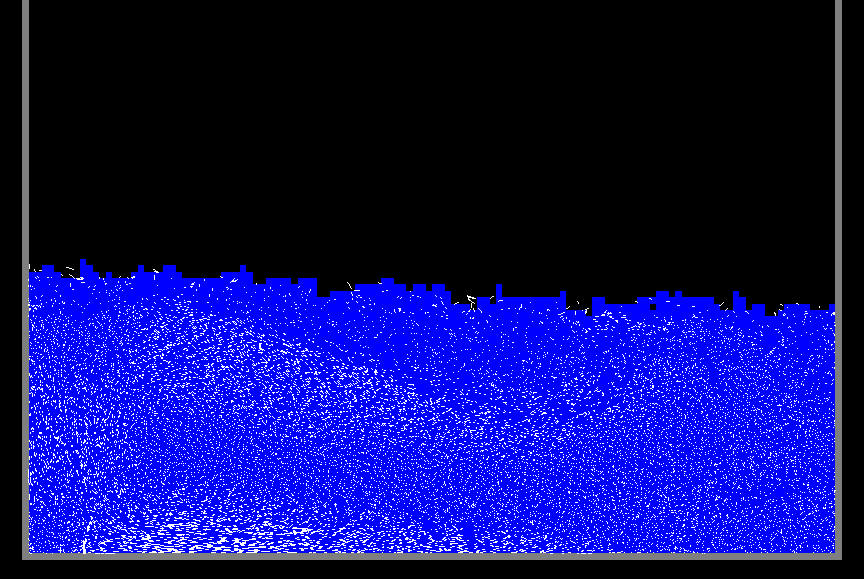
\includegraphics[width=0.40\textwidth]{semilag-perturb-4}
  \caption{Semi-Lagrangian과 PIC Method의 유체 경계의 모양 비교.}
  \label{fluid-boundary}
\end{figure}

Figure \ref{fluid-boundary}은 유체의 진동이 잠잠해 졌을 때 유체의 경계의 모양을 비교한 것이다. Semi-Lagrangian Method의 경우에는 유체의 경계가 매끄럽지 않고 끓어오르는 것 처럼 끊임없이 진동을 하는 반면에, PIC Method의 경우에는 비교적 경계가 부끄럽게 이여지는 것을 알 수 있었다. (참고로 level set을 메시로 변환하여 렌더링했다면 경계를 현재보다 좀 더 매끄럽게 표현할 수 있었을 것이다.)


Figure \ref{realism-semilag}, \ref{realism-pic}에서는 초기 상태 B에서 진폭 2.0$m/s^2$, 주기 2.0s의 좌우로 진동하는 가속도를 주어 시뮬레이션을 수행하였다. 그래프를 보았을 때, Semi-Lagrangian은 좌우로 약간씩 출렁거렸지만, PIC에서는 유체가 심하게 흔들리면서 끊어지고 서로 부딧히는 모습을 볼 수 있었다.

\begin{figure}[h]
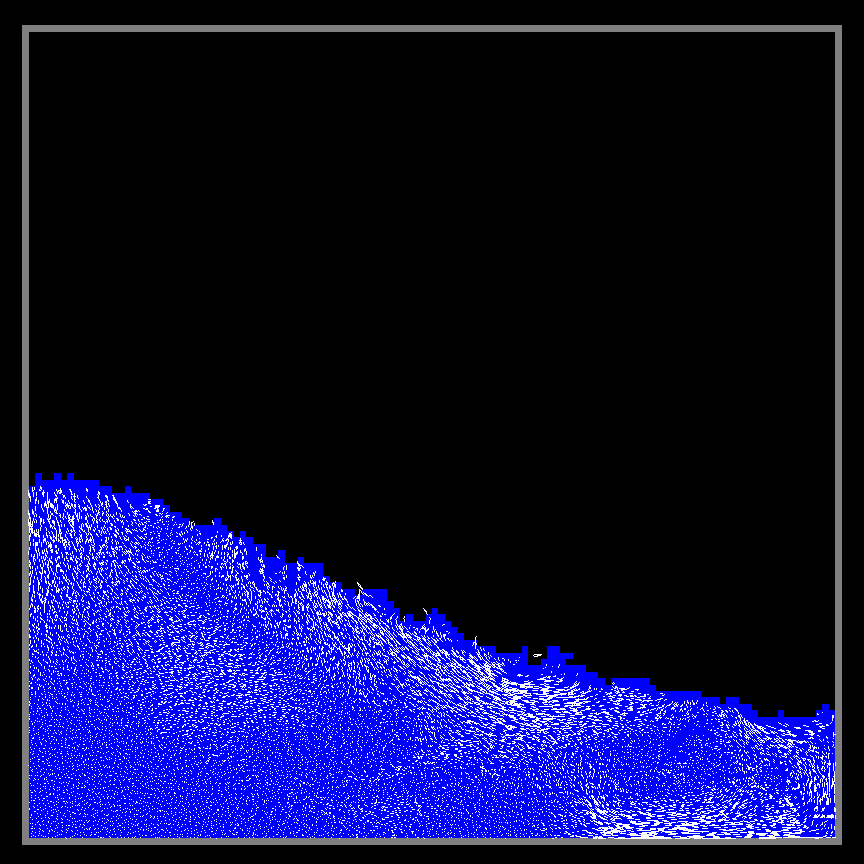
\includegraphics[width=0.24\textwidth]{realism-semilag-1}
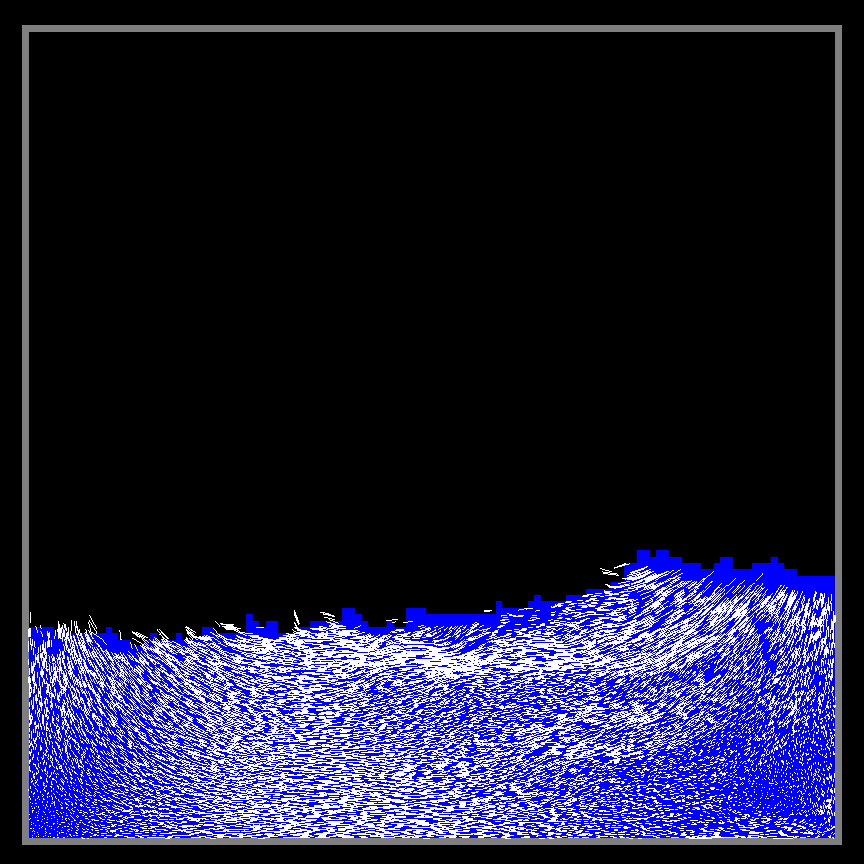
\includegraphics[width=0.24\textwidth]{realism-semilag-2}
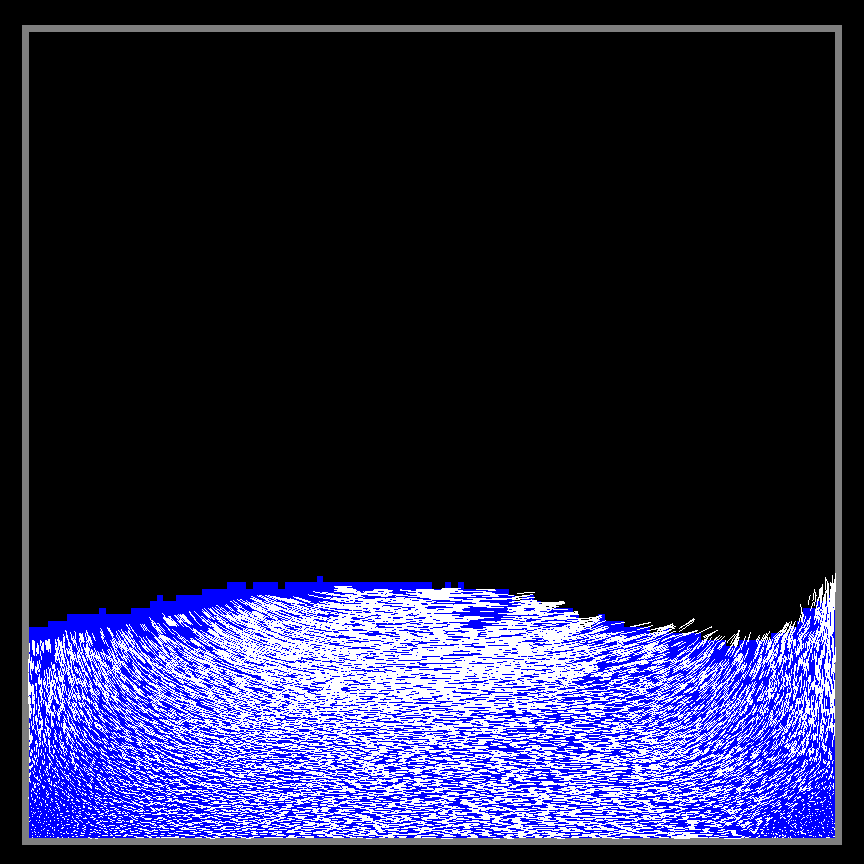
\includegraphics[width=0.24\textwidth]{realism-semilag-3}
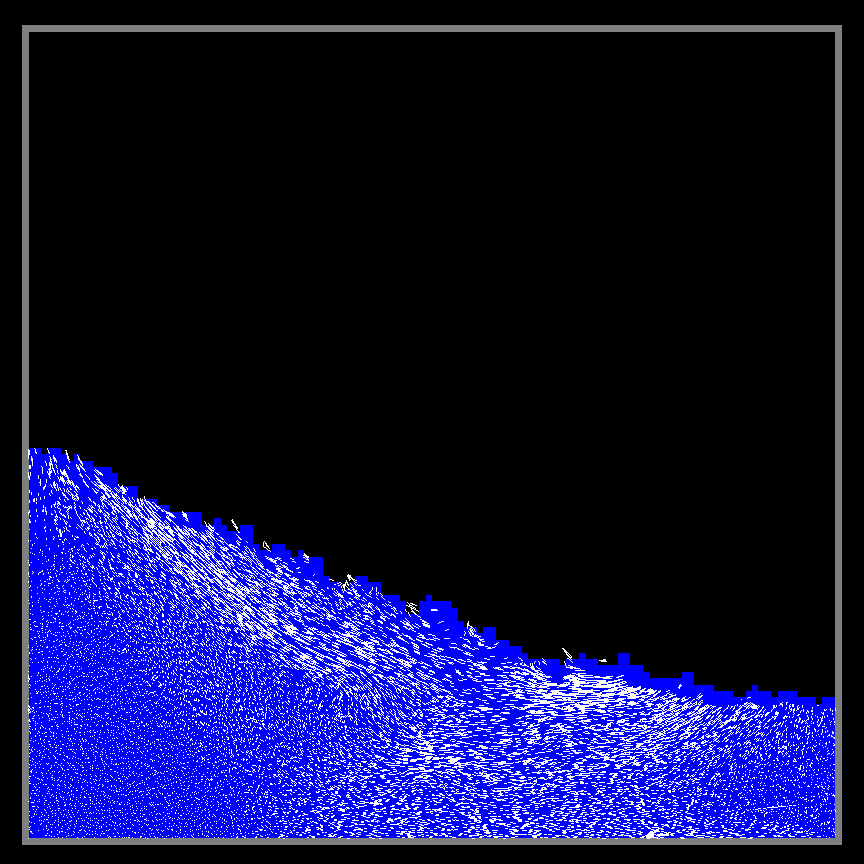
\includegraphics[width=0.24\textwidth]{realism-semilag-4}
  \caption{Semi-Lagrangian Method 예시.}
  \label{realism-semilag}
\end{figure}

\begin{figure}[h]
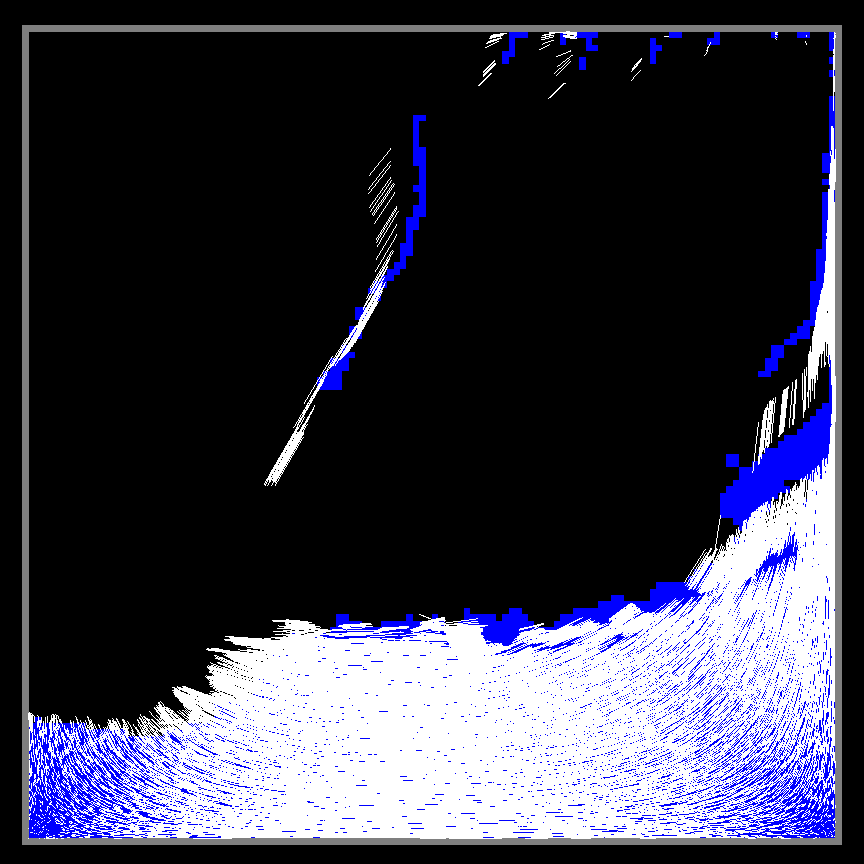
\includegraphics[width=0.24\textwidth]{realism-pic-1}
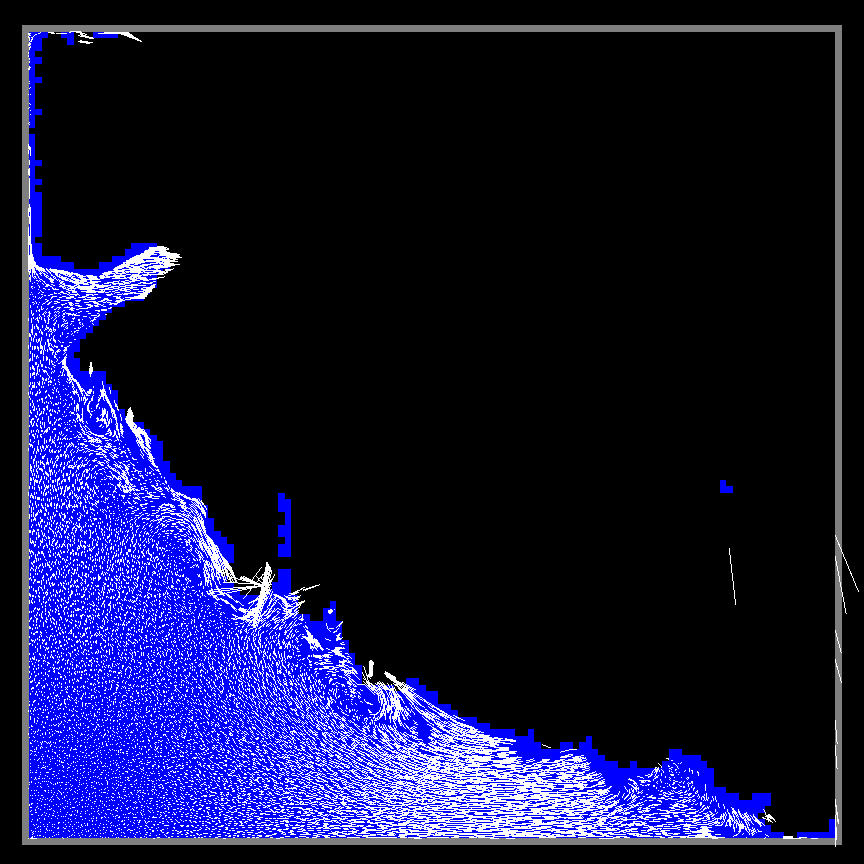
\includegraphics[width=0.24\textwidth]{realism-pic-2}
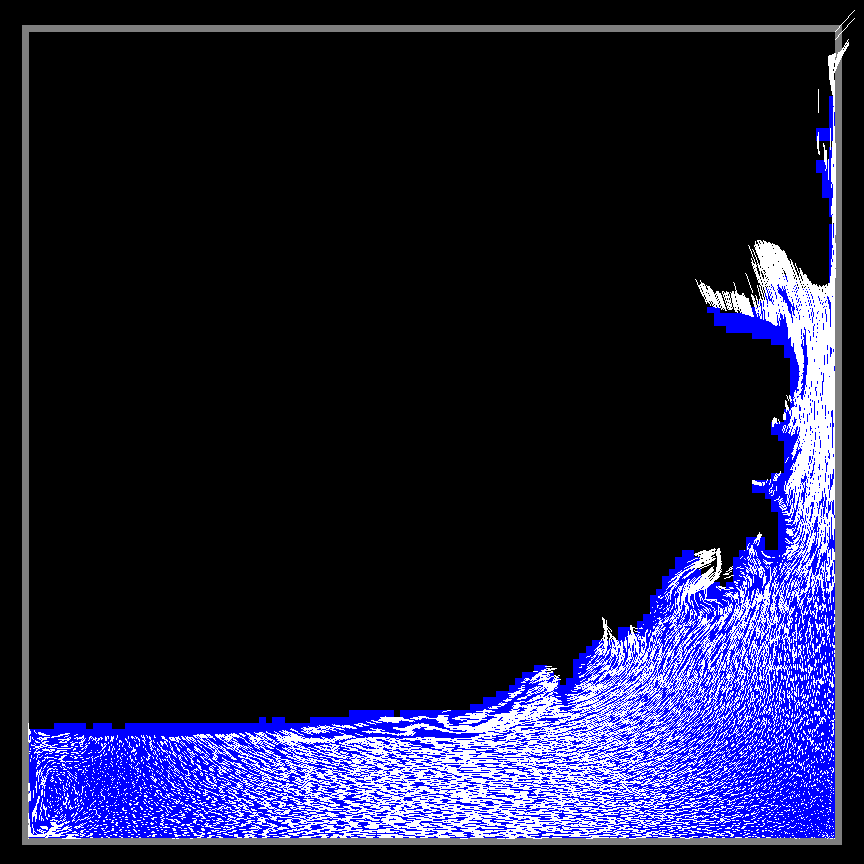
\includegraphics[width=0.24\textwidth]{realism-pic-3}
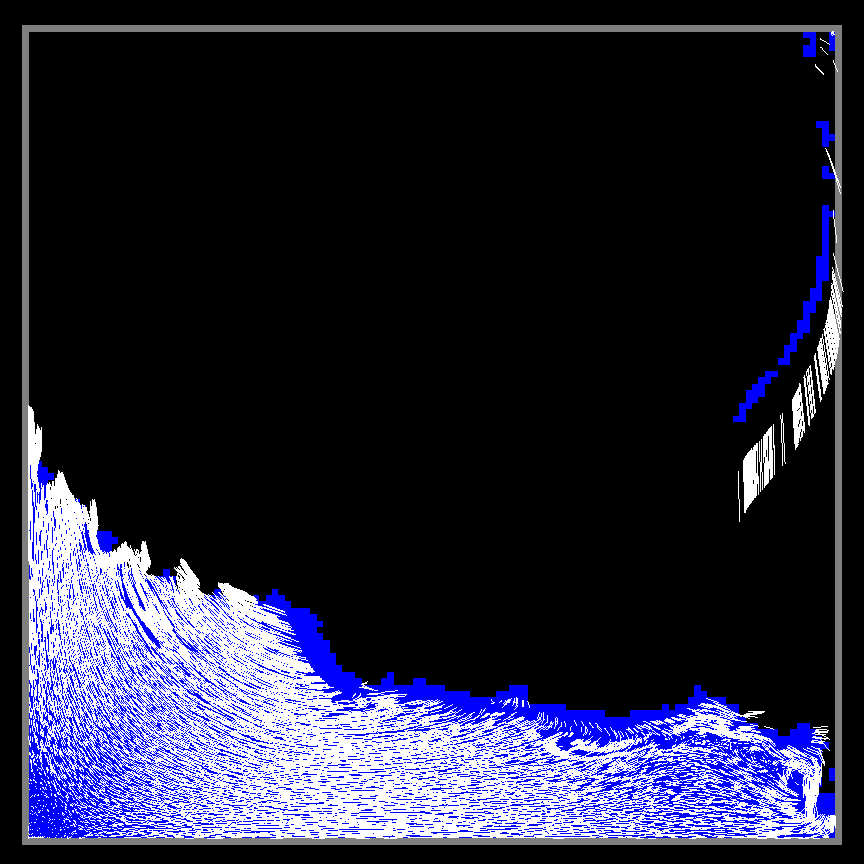
\includegraphics[width=0.24\textwidth]{realism-pic-4}
  \caption{PIC Method ($\alpha$=1.0) 예시.}
  \label{realism-pic}
\end{figure}

PIC와 FLIP의 비중에 따라 유체의 운동이 어떻게 바뀌는지에 대해서도 조사해 보았다. (TODO)

\subsection{Numerical Analysis}

눈으로만 보아서는 유체의 현실성을 평가하기 어렵기 때문에, 이론적으로 유체가 보존해야 하는 물리량들이 시간에 따라 어떻게 바뀌는지를 알아볼 것이다. 일단 유체의 총 부피가 시간에 따라 보존되는지를 확인해 보았다. (PIC Method에서는 PIC와 FLIP의 regularization factor $\alpha$를 바꿔가면서 여러 개의 시뮬레이션을 수행하였다.)

\begin{figure}[h]
  \centering
  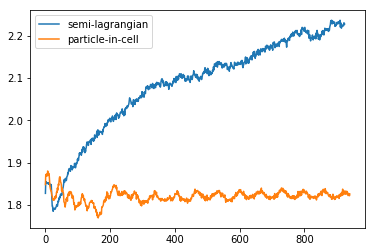
\includegraphics[width=0.7\textwidth]{picflip-volume-graph}
  \caption{PIC Method에서 시간에 따른 부피의 변화. $\alpha$는 PIC/FLIP 사이의 regularization factor이다. }
  \label{volume-increase-graph}
\end{figure}

Figure \ref{volume-increase-graph}의 그래프를 분석하면 대부분의 경우에 대하여 부피가 점점 증가하는 것을 알 수 있었다. (예외라면 $\alpha=0.9$일때 부피가 원래보다 감소하는 경향을 갖는다.) Semi-Lagrangian과 PIC과 비교를 해 보면, 전자가 총 부피가 더욱 많이 증가하는 것을 알 수 있었다. 그리고 $\alpha$값이 작아질수록 (즉 PIC보다 FLIP가 비중이 많아질수록) 부피가 원래보다 더욱 많이 팽창한다는 것을 알 수 있었는데, 오히려 PIC만 사용하고 FLIP를 사용하지 않았을 때 ($\alpha$ = 1.0) 부피 보존이 가장 잘 됨을 확인할 수 있다. 즉 현재로서 FLIP 방법은 부피 보존을 효과적으로 만족시키지 못한다는 것을 알 수 있었다. 

\begin{figure}[h]
  \centering
  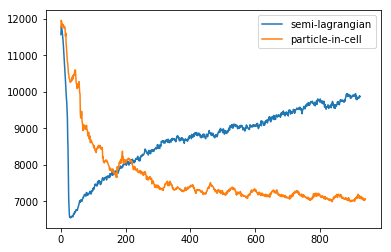
\includegraphics[width=0.4\textwidth]{picflip-energy-graph}
  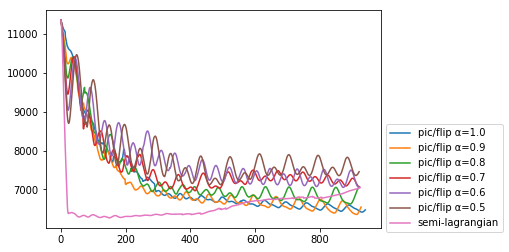
\includegraphics[width=0.52\textwidth]{picflip-particle-energy-graph}
  \caption{PIC Method에서 시간에 따른 총 에너지의 변화. 왼쪽의 그래프에서는 총 에너지를 Grid의 유체 셀들의 에너지를 총합해서 계산했고, 오른쪽의 그래프에서는 유체 파티클들의 에너지를 총합해서 계산했다.}
  \label{energy-graph}
\end{figure}

\begin{figure}[h!]
  \centering
  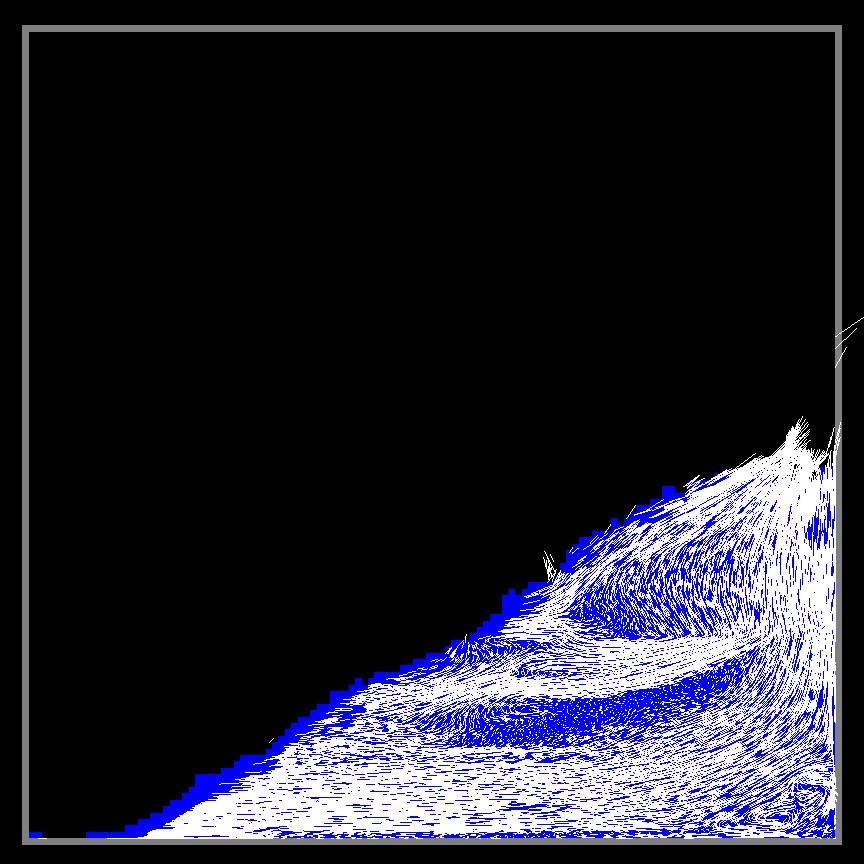
\includegraphics[width=0.19\textwidth]{explode1}
  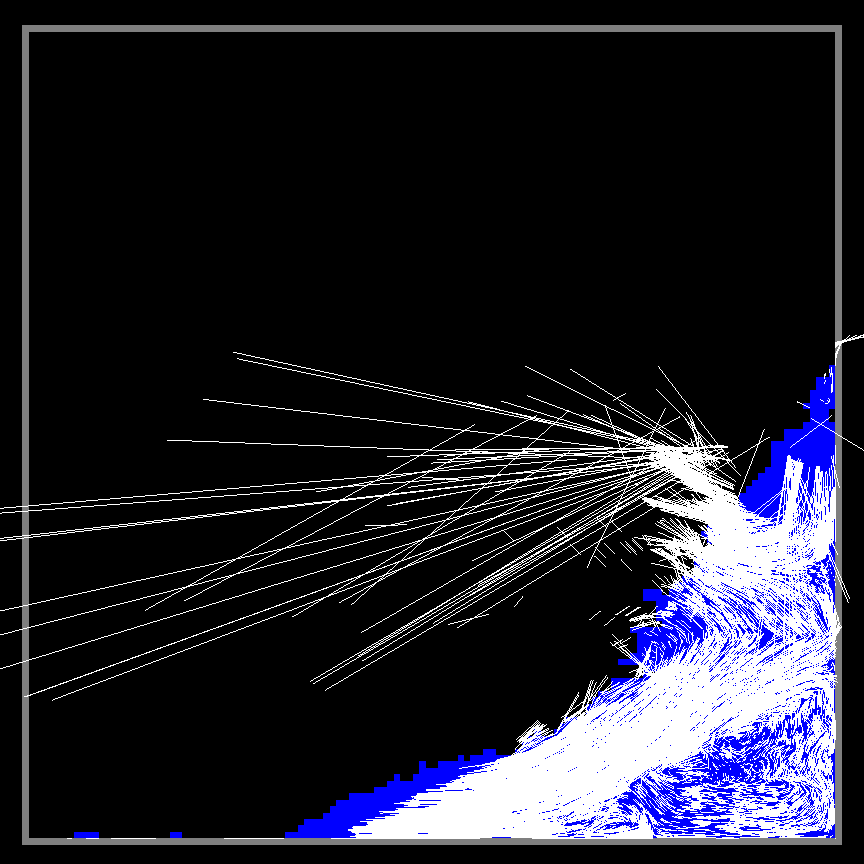
\includegraphics[width=0.19\textwidth]{explode2}
  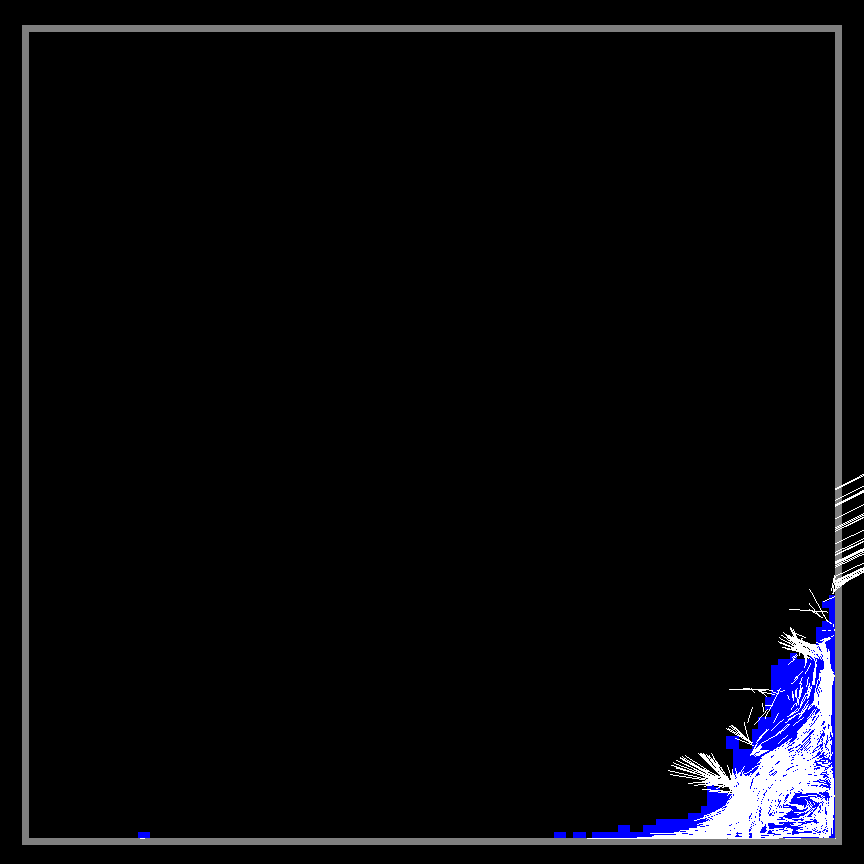
\includegraphics[width=0.19\textwidth]{explode3}
  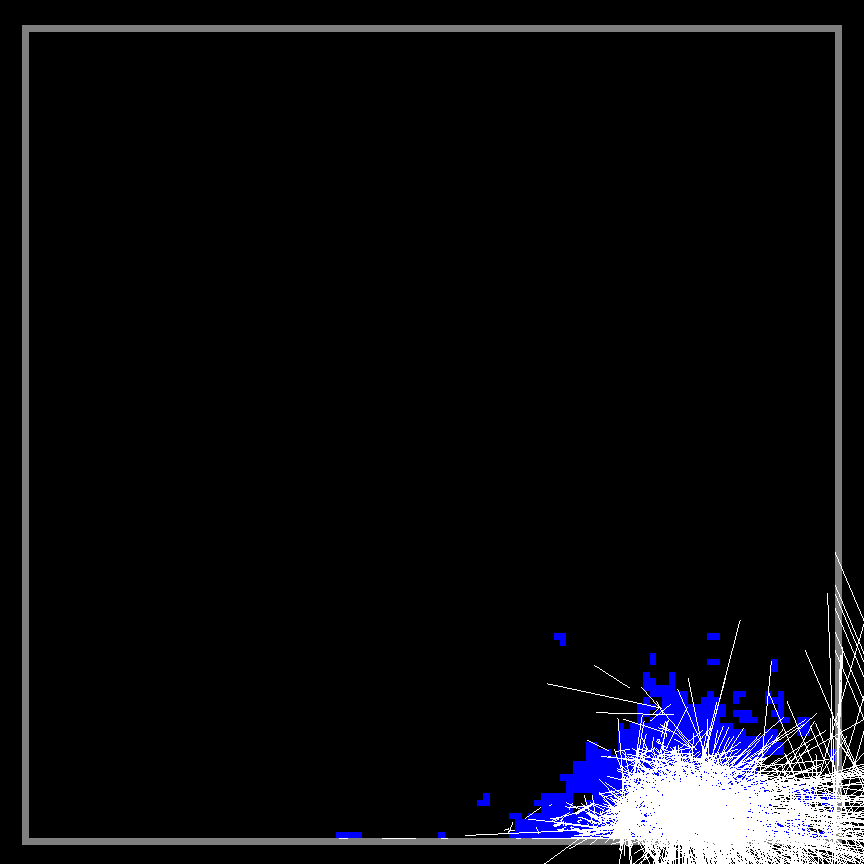
\includegraphics[width=0.19\textwidth]{explode4}
  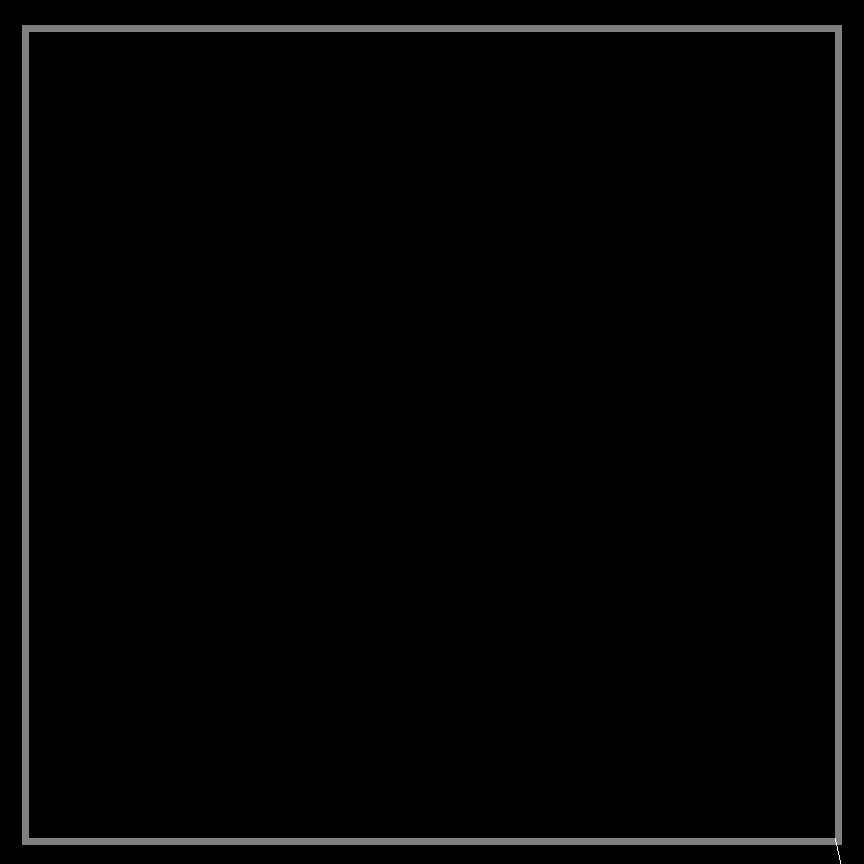
\includegraphics[width=0.19\textwidth]{explode5}
  \caption{가속도가 오른쪽으로 15$m/s^2$, 아래로 9.8$m/s^2$으로 주어졌을 때 파티클들이 모두 한 모서리에 모이게 되는 현상이 일어났다. $\Delta t$ = 0.033s, $\Delta x$ = 0.02m, Semi-Lagrangian Method 사용.}
  \label{explode}
\end{figure}


Figure \ref{energy-graph}의 그래프를 분석하면 시뮬레이션의 초반부에는 어떠한 방법을 사용하든 에너지가 급격히 감소하는 것을 알 수 있다. 하지만 시간이 조금 지나면 PIC Method의 경우에는 진동하면서 일정한 값으로 수렴하게 된다. Semi-Lagrangian 방법의 경우에는 오랜 시간이 지나도 총 에너지가 점점 증가하는 것을 관찰할 수 있었다. 즉 에너지 보존의 관점으로 봤을 때에는 PIC Method가 훨씬 Stable한 방법이다.

\subsection{Instability}

한 방향으로 매우 갑작스러운 강한 힘이 주어져 유속이 매우 빨라졌을 때, Semi-Lagrangian/PIC에 상관없이 시뮬레이션이 불안정해지면서 점점 부피가 감소하는 것을 관찰할 수 있었다. 파티클들의 수가 감소하는 것을 보아 디버거로 파티클들의 위치를 확인했더니, 여러개의 파티클들이 벽면의 모서리 한 곳에 뭉치는 것을 알 수 있었다.  예를 들어서 Figure 11은 Semi-Lagrangian Method에서 가속도가 오른쪽 아래로 크게 주어졌을 때 일어난 현상이다. 

이러한 현상은 Semi-Lagrangian Method 에서 좀 더 심하게 보였으나, PIC Method에서도 비슷하게 재현할 수 있었다. 특히 timestep ($\Delta t$)가 높은 상황에서 이것이 일어날 가능성이 더 높았다.
 
\subsection{Performance}

\begin{table}[h]
\centering
\begin{tabular}{|l|l|l|l|l|}
\hline
                & A     & B     & C     & Average \\ \hline
Semi-Lagrangian & 31.32 & 27.32 & 26.51 & 28.38   \\ \hline
PIC/FLIP        & 24.57 & 20.91 & 19.09 & 21.52   \\ \hline
\end{tabular}
\caption{초기 상태 A, B, C에서 각각 Semi-Lagrangian과 PIC Method를 사용했을 때의 한 프레임당 시뮬레이션 연산 시간 (단위는 ms. 조건: $\Delta t$ = 0.033s, $\Delta x$ = 0.02m, 그리드 크기는 128x128.)}
  \label{performance}
\end{table}

결과적으로는 128x128의 그리드 크기에 대해 노트북 CPU에서도 실시간으로 (30FPS 이상) 돌아가는 유체 시뮬레이션을 수행할 수 있었다. Table \ref{performance}은 Semi-Lagrangian과 PIC Method의 성능을 각각 다른 초기 조건 A, B, C에서 측정한 결과이다. (참고: 본 성능측정은 Intel(R) Core(TM) i7-6700HQ CPU (Quad core, Hyperthreading, 2.60Ghz)에서 진행했으며, 처음 30초 동안 프로그램을 돌렸을 때의 한 프레임 당 유체 시뮬레이션 코드가 걸린 전체 시간의 평균을 구한 것이다.)

결과적으로 Semi-Lagrangian이 PIC/FLIP보다 연산시간이 많이 걸렸다. 이것의 이유로는 Semi-Lagrangian 방법의 Advection Step에서 3rd order Runge-Kutta를 사용했는데, 이것을 수행하려면 한 셀당 bicubic interpolation을 총 6번 수행해야 했기 때문이다. 반면에 PIC/FLIP method에서는 Runge-Kutta 대신에 grid-to-particle, particle-to-grid transfer를 수행해야 했는데, 이 때는 bilinear sampling을 사용해서 연산량이 비교적 덜 소모되었다. (수치로 확인하면 Semi-Lagrangian advection은 0.922ms, grid-to-particle와 particle-to-grid transfer는 각각 0.447ms이 걸렸다.) 이것 이외에도 Semi-Lagrangian와 PIC의 Pressure Update 시간이 각각 4.41ms과 3.68ms가 걸려, PIC/FLIP에서 MICCG 알고리즘이 좀 더 빨리 수렴한다는 것을 알 수 있다.

\section{Discussion}

\subsection{Explanation of Results}

결과 중에서 눈여겨 볼 점은 Semi-Lagrangian이 PIC보다 부피와 에너지 보존 측면에서 안 좋았다는 것이다. 특히 Semi-Lagrangian의 부피 팽창 현상이 심한 것을 눈여겨 볼 수 있다. 이것에 대한 해석으로는, 논문의 사진으로는 잘 보이지 않지만 운동이 비교적 많이 일어나는 표면 근처의 셀들에서 파티클 밀도가 감소하는 것을 관찰할 수 있었다. 즉 표면의 활발한 파티클들이 서로 분산되면서 차지하고 있는 셀들의 밀도값이 낮아지는데, 이것이 유체 시뮬레이션의 어떠한 부분에도 보정되지 않아서 문제가 생긴 것이다. 만약에 파티클 밀도에 대한 보정을 가할 수 있다면, Semi-Lagrangian Method의 부피 팽창 문제를 해결할 수 있을 것이다. (방법은 \textbf{Further Improvements}를 참조하자.)

Figure \ref{energy-graph} 의 Semi-Lagrangian 방법에서 (처음의 에너지 감소를 제외하고) 총 에너지가 점점 증가하는 이유는, 현재 부피가 점점 커지고 있기 때문에 셀 단위로 에니지 계산을 수행하면 부피에 비례하여 에너지가 증가할 수 밖에 없기 때문이다.

Semi-Lagrangian과 PIC에서의 총 에너지 감소가 일어나는 원인에 대해 살펴보자. 그래프를 보면 처음에만 에너지가 급격하게 감소하다가 조금 뒤에는 일정해지는 것을 알 수 있다. (PIC의 경우에는 시간이 지나면 특정한 에너지 값을 중심으로 조금씩 진동하는 것을 알 수 있다.) 대부분의 에너지 감소가 처음에 이루어지는 이유는, 시뮬레이션의 초반부에 물이 고체 벽에 높은 속도로 부딪히면서, 벽에서의 유체의 Boundary Condition을 만족시켜야 하기 때문에 벽과 수직 방향의 속도가 갑자기 0이 되기 때문이다. 즉 시뮬레이션에서는 물의 충격량을 벽이 모두 흡수하도록 되어 있기 때문에, 총 에너지가 감소할 수 밖에 없는 것이다. 초반을 제외한다면 양쪽 방법에서 에너지 보존이 어느 정도는 지켜지고 있다는 것을 그래프에서 알 수 있다.

\subsection{Further Improvements}

현재의 프로그램에서 Semi-Lagrangian 방법과 PIC Method 모두 부피가 증가/감소하는 현상을 관찰할 수 있었다. (특히 Semi-Lagrangian 방법에서는 부피 팽창이 심한 것을 측정하였다.) 이것을 해결한다면 파티클이 부족한 셀에 새로운 파티클을 추가하고, 파티클이 너무 많은 셀에 파티클을 제거하는 reseeding stage를 추가하는 것이 효과가 있을 것이다. \cite[p. 117]{fluid-sim-cg} 물론 reseeding에서 파티클의 수는 일정하게 유지되게 해야 할 것이다. 더욱 정확한 분배를 하고 싶다면 유체의 level set을 사용하여 경계를 찾은 다음 유체의 안쪽에 파티클들을 골고루 분배할 수 있을 것이다.  혹은 Kim et al. \cite{volume-preservation} 의 논문의 방법처럼 projection step에서 velocity field의 divergence를 0이 아닌 다른 값으로 보정해 해결하는 방식도 있다. \textbf{Result} 섹션에서 언급했던 파티클이 하나의 모서리로 모이는 문제도 reseeding을 통해 해결할 수 있을 것으로 보인다.

현재의 유체 시뮬레이션에서 개선할 점이 있다면, Pressure Solver의 numerical stability를 개선하는 것이다. 파티클의 속도가 굉장히 높아지는 극단적인 경우에 대해 Pressure Solver가 수렴을 하지 못해 올바른 해를 찾지 못하는 경우가 관찰되었는데, 실제로 산업에서 활용할 만한 기술로 만든다면 다양한 상황에 대해서도 무리 없이 돌아가도록 고쳐야 할 것이다. 이를 해결할 수 있는 방법 중 하나는 특정 파티클들의 속도가 너무 빨라지면 해당되는 파티클의 integration을 하는 timestep의 크기 ($\Delta t$) 를 유동적으로 줄이는 것이다. \cite[p. 35]{fluid-sim-cg} 또 다른 해결 방안은 MICCG의 두 패러미터 값 $\tau$, $\sigma$를 fine tuning해 더욱 좋은 수치를 찾는 것이다. (현재는 $\tau=0.999$, $\sigma=0.25$을 사용하고 있다.)

이것 외에도 PIC와 FLIP을 더욱 개선할 수 있는 APIC (Affine Particle-in-cell) 방법이 있는데, PIC에서의 dissipation이 일어나는 현상과 FLIP의 불안정성을 동시에 해결할 수 있는 방법이다. \cite{apic}

\section{Conclusion}

우리는 그리드 기반 2D 유체 애니메이션을 두 가지 접근법 (Semi-Lagrangian, Particle-in-cell)을 사용하여 제작할 수 있었고, 이를 실시간으로 돌릴 수 있었다. 결과적으로 Particle-in-cell이 Semi-Lagrangian 방법보다 유체의 역동적인 모습을 효과적으로 재현할 수 있었다. Particle-in-cell method의 경우에는 PIC와 FLIP을 혼용하여 사용했을 때, 총 에너지의 변화를 보아 FLIP이 dissipation을 줄여주는 역활을 하긴 하지만, 순수 PIC의 역동적인 모습을 재현하진 못한다는 것을 알 수 있었다. 현재의 구현체는 Volume preservation을 만족하지 못하는 문제가 있지만, 이를 particle reseeding 등의 방법을 통해 해결할 수 있을 것이다.


\begin{thebibliography}{9}
\bibitem{fluid-sim-cg}
Robert Bridson.
\textit{Fluid Simulation for Computer Graphics, Second Edition}. 
A K Peters/CRC Press, 2015.

\bibitem{dist-function}
Yen-hsi Richard Tsai,
\textit{Rapid and Accurate Computation of the Distance Function Using Grids}
Journal of Computational Physics, Volume 178, Issue 1, p. 175-195, 2002.

\bibitem{fast-sweeping}
Zhao, Hongkai.
\textit{A fast sweeping method for Eikonal equations}.
Mathematics of Computation, 74 (250): p. 603–627, 2005.

\bibitem{flip-fluids}
J.U.Brackbill, D.B.Kothe, H.M.Ruppel.
\textit{FLIP: A Low-dissipation, Particle-in-cell Method for Fluid Flow}.
Computer Physics Communications, 48, p. 25-38, 1988.

\bibitem{volume-preservation}
Kim, Byungmoon and Liu, Yingjie and Llamas, Ignacio and Jiao, Xiangmin and Rossignac, Jarek
\textit{Simulation of Bubbles in Foam with the Volume Control Method}
ACM Trans. Graph., 26.3, 2007.

\bibitem{apic}
Chenfanfu Jiang, Craig Schroeder, Andrew Selle, Joseph Teran, and Alexey Stomakhin.
\textit{The affine particle-in-cell method}.
ACM Trans. Graph., 34.4, Article 51, 2015.
\end{thebibliography}

\end{CJK}

\end{document}
